\section{Evaluation}
\label{sec:evaluation}

In this section we evaluate the proposed scheme through experiments on 
Flash chips. In addition to validating correct operation of the 
encoding and decoding algorithms, we also study the robustness across 
various design parameters, performance, detectability, recovery 
without the hiding key, and erase tolerance.

\subsection{Evaluation Setup}

\subsubsection{Testbed Device}

\begin{figure}
\begin{center} 
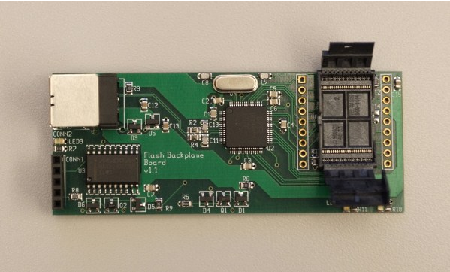
\includegraphics[width=\mywidth]{figs/flashtestboard.pdf} 
\caption{Flash test board.}
\label{fig:flashtestboard} 
\vspace{-0.1in}
\end{center} 
\end{figure} 

Our experiments use a custom Flash test board as shown in 
Figure~\ref{fig:flashtestboard}. The board is made entirely with 
commercial off-the-shelf (COTS) components with a custom PCB. 
There is a socket to hold a Flash chip under test, an ARM 
microprocessor to issue commands and receive data from the Flash 
chip, and a Maxim MAX-3233 chip to provide a serial (RS-232) 
interface. USB support is integrated into the ARM microcontroller. 
We also wrote the code to test the device. The setup represents 
typical small embedded platforms such as USB Flash drives, sensor 
nodes, etc. This device shows that the techniques can be applied 
to commercial off-the-shelf devices with no custom integrated 
circuits (ICs).

\subsubsection{Flash Memory Chips}

\begin{table}
  \begin{center}
    %\begin{scriptsize}
\begin{tabular}{|l|l|r|r|r|}
\hline

{\bf Manufacturer}& {\bf Part Number} & {\bf Size} & {\bf Qty} & {\bf Process} \\

\hline
Hynix & HY27UF084G2B & 4 Gbit & 1 & 5xnm class\\
       & & & & SLC\\
\hline
Micron & MT29F2G08ABA & 2 Gbit & 5 & 34nm \\
       & EAWP-IT:E4 & & & SLC\\
\hline
Micron & MT29F4G08ABA & 4 Gbit & 15 & 34nm \\
       & DAWP:D & & & SLC\\
\hline
Micron & MT29F16G08CB & 16 Gbit & 1 & -- \\
       & ACAWP:C & & & MLC\\
\hline
Numonyx & NAND04GW & 4 Gbit & 1 & 57nm \\
& 3B2DN6 & & & SLC\\
 
\hline

\end{tabular}
%\end{scriptsize}


  \end{center}
\caption{Tested Flash chips.}
\vspace{-0.2in}
\label{tab:testedchips}
\end{table}

The experiments in this paper were performed with five types of 
Flash memory chips from Numonyx, Micron, and Hynix. 
Table~\ref{tab:testedchips} shows their details. 
We primarily performed experiments with Micron 4Gbit chips.
Experiments using other models will be marked.

In most experiments, we only used the first 4,096 bits of 16,896-bit pages to
avoid performance overheads given the limited amount of memory in the microcontroller.
We will refer to the first 4,096 bits as a ``page'' in the following discussion.
For the analyses of per-page read/program time and per-block erase time, we
used the entire page.


%\subsection{Overall Operation}

%WE MAY REMOVE THIS SUBSECTION.

%\begin{figure} 
%\begin{center} 
%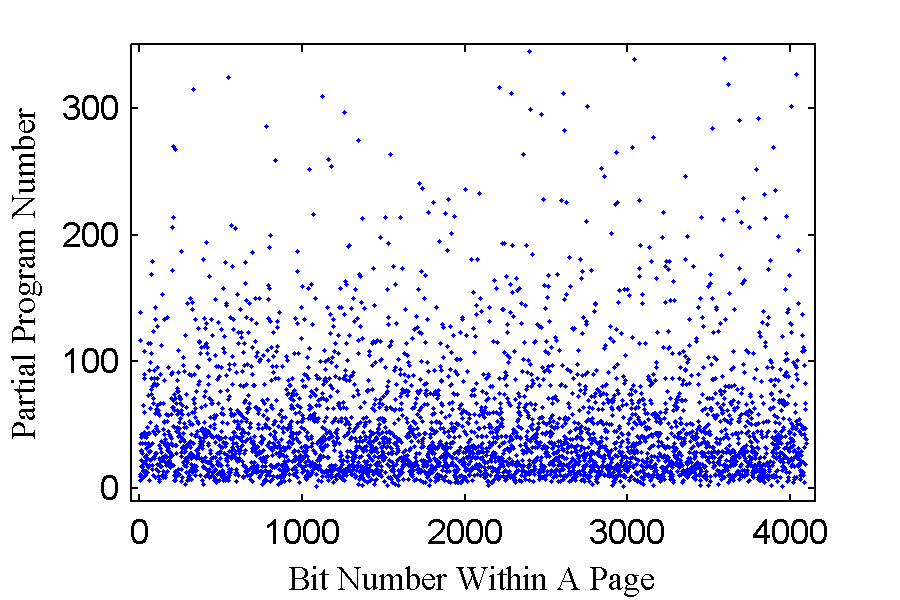
\includegraphics[width=\mywidth]{figs/program_numbers_c1_5e3pe_block1_page0.png} 
%%\includegraphics[width=3.0in]{figs/eval_performance_diff_context.pdf} 
%\caption{Raw partial program numbers for bits in a page.}
%\vspace{-0.1in}
%\label{fig:ptimeraw} 

%\end{center} 
%\end{figure} 


%\begin{figure} 
%\begin{center} 
%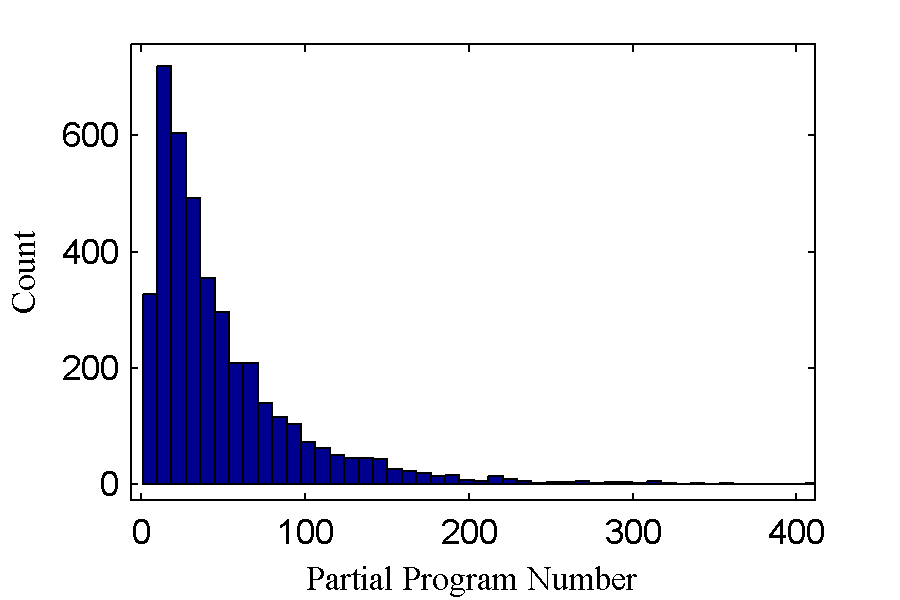
\includegraphics[width=\mywidth]{figs/hist_c1_block1_page1.png} 
%%\includegraphics[width=3.0in]{figs/eval_performance_diff_context.pdf} 
%\caption{Partial program time distribution for bits in a page.}
%\vspace{-0.1in}
%\label{fig:ptimehisto} 

%\end{center} 
%\end{figure} 

%Figure~\ref{fig:ptimeraw} shows the raw program numbers for the 
%bits in a page with hidden information. The program time distribution 
%is shown in Figure~\ref{fig:ptimehisto}. The first 4,096 bits of the 
%page are used and 
%they are divided into 32 groups randomly based on the stego-key.
%5,000 program and erase cycles are applied in the encoding process. 
%Even though bits are intentionally stressed 5,000 times, as the figures
%show, there is no obvious bi-modal distribution between fast and slow
%bits. This results indicates that the inherent variation in program time
%across bits is much greater than the stress induced changes. The 
%distributions do not show a clear sign of hidden bits.

%No obvious bi-modal behavior, which could highlight our stressed pages, 
%is observed in Figure~\ref{fig:ptimehisto}. 


% \begin{figure} 
% \begin{center} 
% 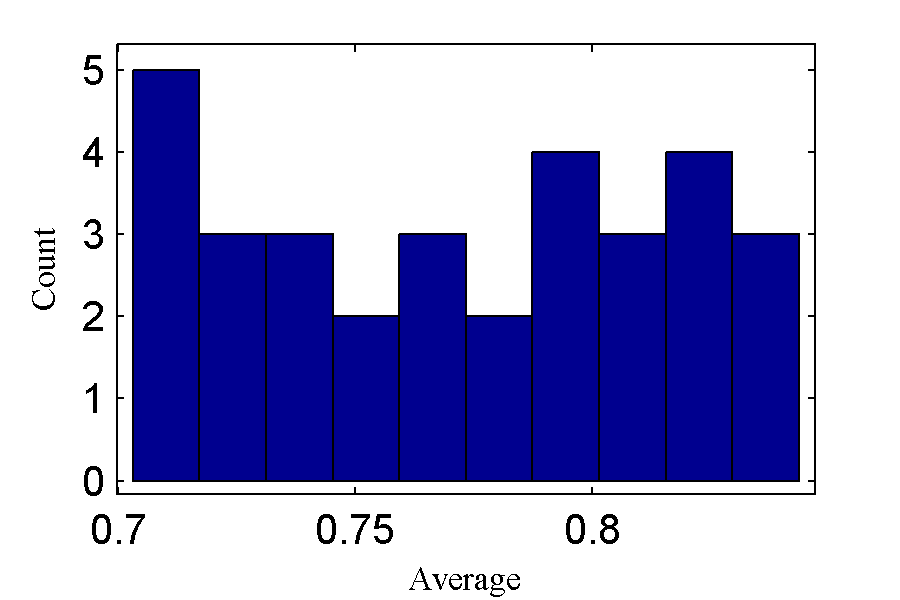
\includegraphics[width=\mywidth]{figs/hist_c1_block1_page1_withoutkey.png} 
%\includegraphics[width=3.0in]{figs/eval_performance_diff_context.pdf} 
% \caption{Group average without the stego-key}
% \label{fig:withoutkey_page} 

% \end{center} 
% \end{figure} 

% \begin{figure} 
% \begin{center} 
% 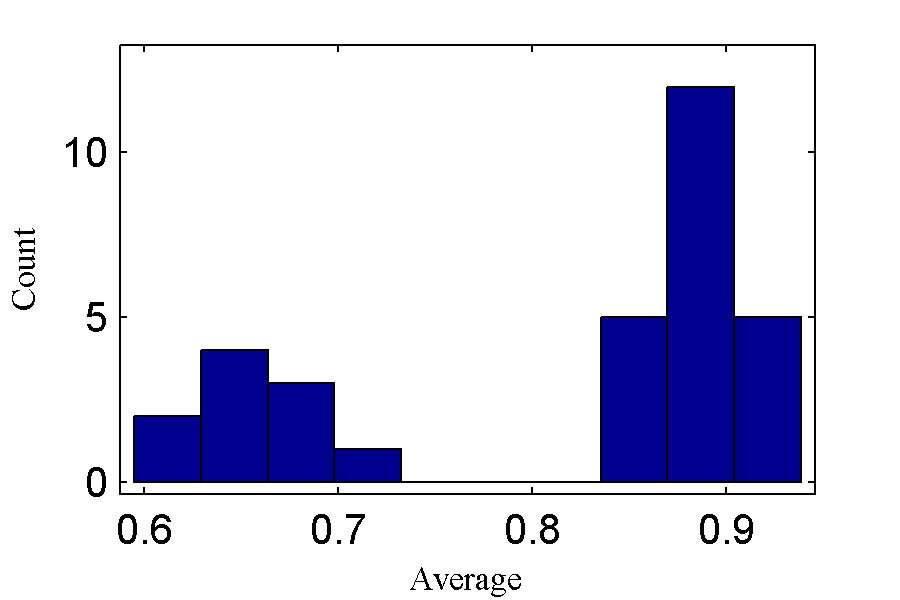
\includegraphics[width=\mywidth]{figs/hist_c1_block1_page1_withkey.png} 
%\includegraphics[width=3.0in]{figs/eval_performance_diff_context.pdf} 
% \caption{Group average with the stego-key}
% \label{fig:withkey_page} 

% \end{center} 
% \end{figure} 

%\begin{figure} 
%\begin{center} 
%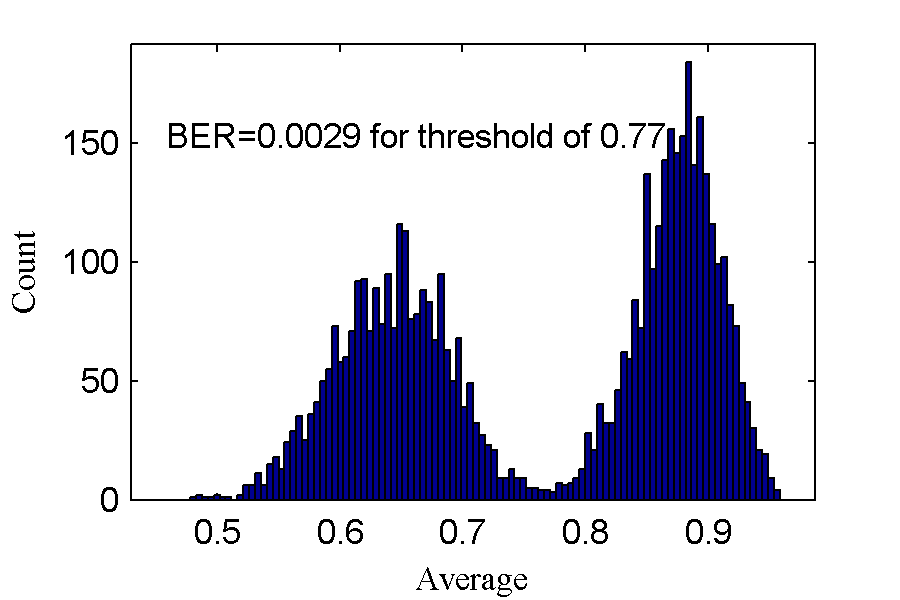
\includegraphics[width=\mywidth]{figs/5e3_histo_withkey.png} 
%%\includegraphics[width=3.0in]{figs/eval_performance_diff_context.pdf} 
%\caption{The distribution of the average program time of a group with 
%the stego-key.}
%\label{fig:withkey_10blocks} 
%\vspace{-0.1in}
%\end{center} 
%\end{figure} 

%To recover hidden information from the program time distribution,
%the intended recipient with the stego-key can compute the average
%program time for each group after the first thresholding. 
%Figure~\ref{fig:withoutkey_10blocks} shows the distribution of
%the resulting average program time.
%In this figure, 5120 groups which represent 5120 embedded bits
%are shown. 
%As shown in the figure, these is an obvious gap in the distribution
%between the fast and slow groups. Therefore, the value of hidden bits 
%can be easily recovered through a simple thresholding. 
%We get a bit error rate (BER) of 0.0029 (0.29\%) in this case.
%%even when a single
%%quantization threshold ($X$) is used across all pages.

%To recover hidden information from the program time distribution,
%the intended recipient with the stego-key can compute the average
%program time for each group after the first thresholding. 
%Figure~\ref{fig:withoutkey_10blocks} shows the distribution of
%the resulting average program time.
%In this figure, 5120 groups which represent 5120 embedded bits
%are shown. 
%As shown in the figure, these is an obvious gap in the distribution
%between the fast and slow groups. Therefore, the value of hidden bits
%can be easily recovered through a simple thresholding. 
%We get a bit error rate (BER) of 0.0029 (0.29\%) in this case.
%%even when a single
%%quantization threshold ($X$) is used across all pages.


%\begin{figure} 
%\begin{center} 
%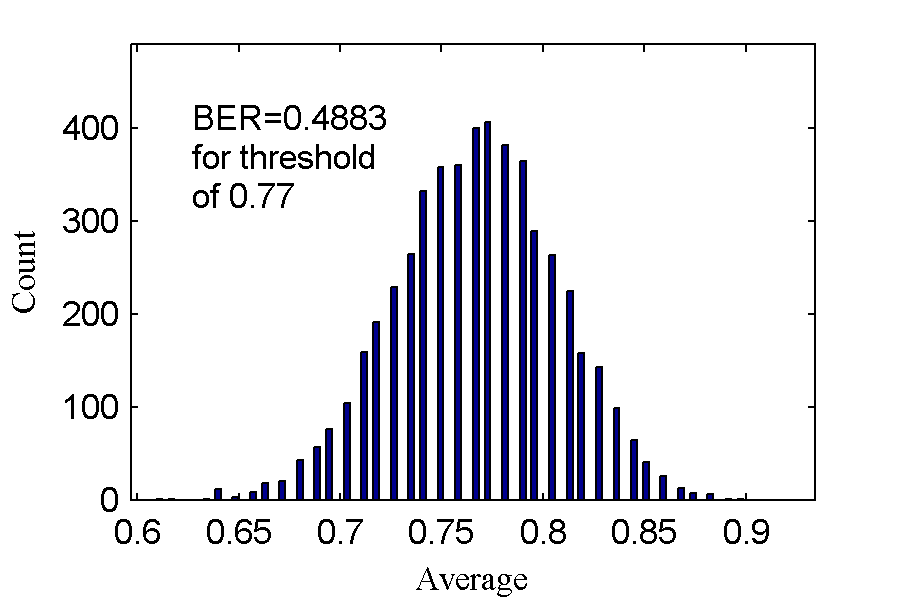
\includegraphics[width=\mywidth]{figs/5e3_histo_withoutkey.png} 
%%\includegraphics[width=3.0in]{figs/eval_performance_diff_context.pdf}
%\caption{The distribution of the average program time of a group
% without the stego-key.}
%\label{fig:withoutkey_10blocks} 
%\vspace{-0.1in}
%\end{center} 
%\end{figure} 

%On the other hand, Figure~\ref{fig:withoutkey_10blocks} shows the 
%distribution of the average program time when the stego-key is 
%unknown. In this experiment, we randomly selected groups. As shown 
%in the figure, the average program time of a group shows a normal 
%distribution without any clear separation between 1s and 0s. The BER 
%with the threshold $Th$ of 0.77 is 0.4883, which is close to 50\%. 
%This result suggests that an adversary cannot recover hidden 
%information without correct groupings because each group is likely 
%to have both more and less stressed bits.



%\begin{figure} 
%\begin{center} 
%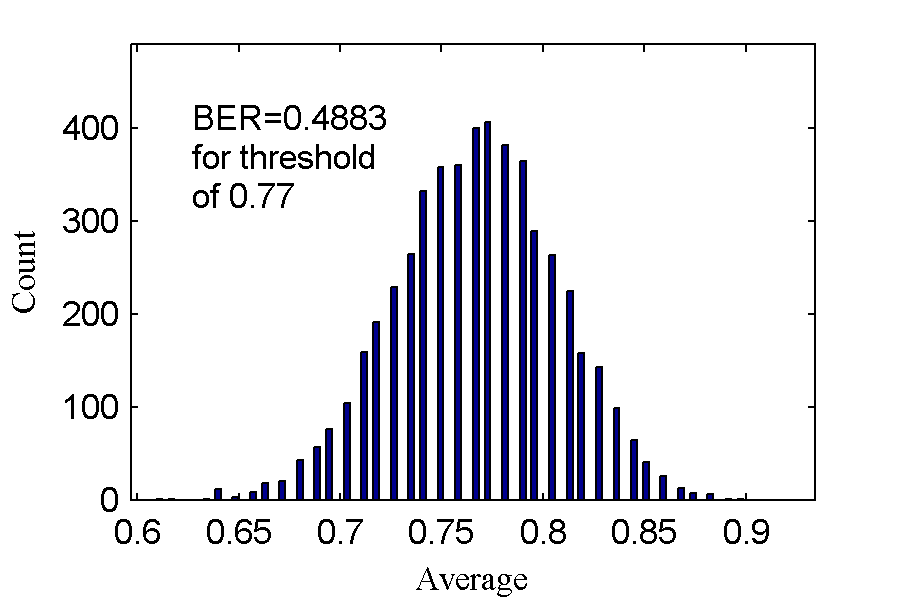
\includegraphics[width=\mywidth]{figs/5e3_histo_withoutkey.png} 
%%\includegraphics[width=3.0in]{figs/eval_performance_diff_context.pdf} 
%\caption{The distribution of the average program time of a group 
%without the stego-key.}
%\label{fig:withoutkey_10blocks} 
%\vspace{-0.1in}
%\end{center} 
%\end{figure} 

%On the other hand, Figure~\ref{fig:withoutkey_10blocks} shows the 
%distribution of the average program time when the stego-key is 
%unknown. In this experiment, we randomly selected groups. As shown
%in the figure, the average program time of a group shows a normal
%distribution without any clear separation between 1s and 0s. The BER
%with the threshold $Th$ of 0.77 is 0.4883, which is close to 50\%. 
%This result suggests that an adversary cannot recover hidden 
%information without correct groupings because each group is likely to
%have both more and less stressed bits.


\subsection{Robustness - Bit Error Rate}

In this subsection, we first study whether the proposed scheme can 
reliably hide and recover bits in the program time characteristics.
Here, we use the bit error rate (BER) as the metric for measuring 
robustness. To measure the BER, we hid a randomly generated message
into Flash memory and compared the retrieved message with the original.

In the baseline experiment, we used the first 4,096 bits of a page and
divided them into 32 groups (128 bits each) based on a randomly 
selected hiding key. Then, we selected multiple pages and blocks across
a Flash chip to form 5,120 groups, which represent 5,120 hidden bits,
and stored bits using 5,000 program and erase (PE) cycles in the encoding 
process. 
%Even though bits are intentionally stressed 5,000 times, as the figures
%show, there is no obvious bi-modal distribution between fast and slow
%bits. This results indicates that the inherent variation in program time
%across bits is much greater than the stress induced changes. The 
%distributions do not show a clear sign of hidden bits.
In this case, we got a bit error rate (BER) of 0.0029 (0.29\%).
%even when a single quantization threshold ($X$) is 
%used across all pages.

\begin{figure} 
\begin{center} 
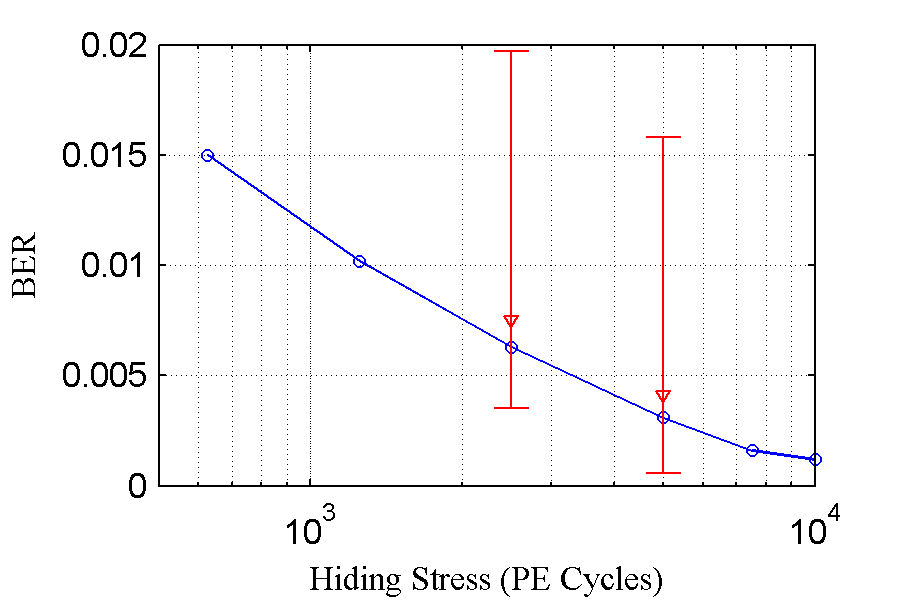
\includegraphics[width=\mywidth]{figs/accuracy.png} 
\caption{Influence of hiding stress on BER.}
\label{fig:BER_vs_stress} 
\vspace{-0.1in}

\end{center} 
\end{figure}


Figure~\ref{fig:BER_vs_stress} shows the BER as a function of 
hiding stress, which is the number of program/erase (PE) cycles used
to stress each group in the hiding process. 
The blue line shows the average BER using a single Micron 4Gbit chip.
For each data point in the figure, the BER is computed over 5,120 
bits of hidden information with the group size of 128 bits.
For hiding stress levels of 2,500 and 5,000 PE cycles, we also show
the statistics across 15 Flash chips; the red triangles show the 
average BER and the error bars show the maximum and minimum BERs across 
the 15 chips. We can see that the BER decreases as the hiding stress 
increases. More stress increases the program time difference between
bits hiding 1s and 0s. However, the incremental benefit after 
5,000 PE cycles is rather small. Note that the typical lifetime
of an SLC Flash chip from the datasheet is 100,000 PE cycles. 

\begin{figure} 
\begin{center} 
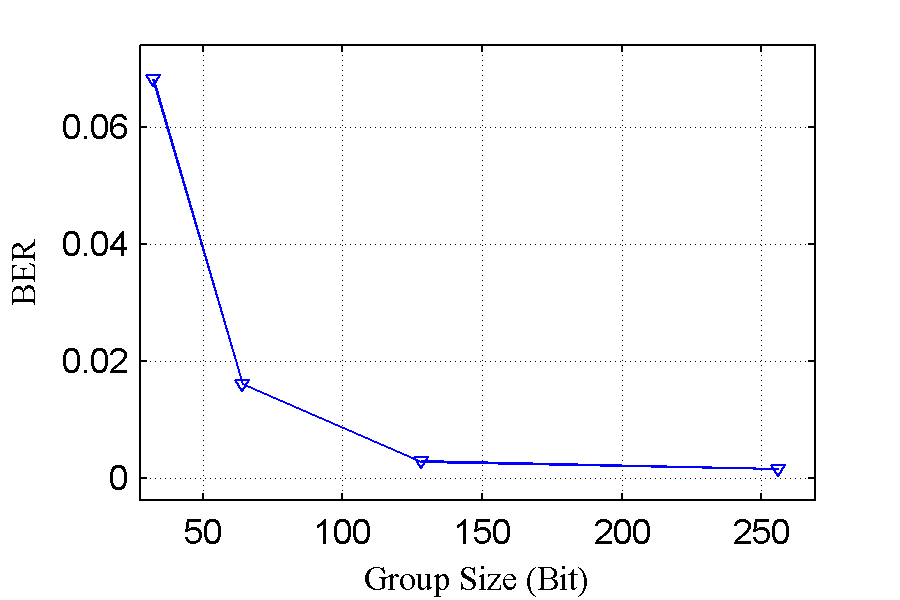
\includegraphics[width=\mywidth]{figs/groupsize.png} 
\caption{Influence of group size on BER.}
\label{fig:groupsize} 
\vspace{-0.1in}

\end{center} 
\end{figure}


\begin{figure} 
\begin{center} 
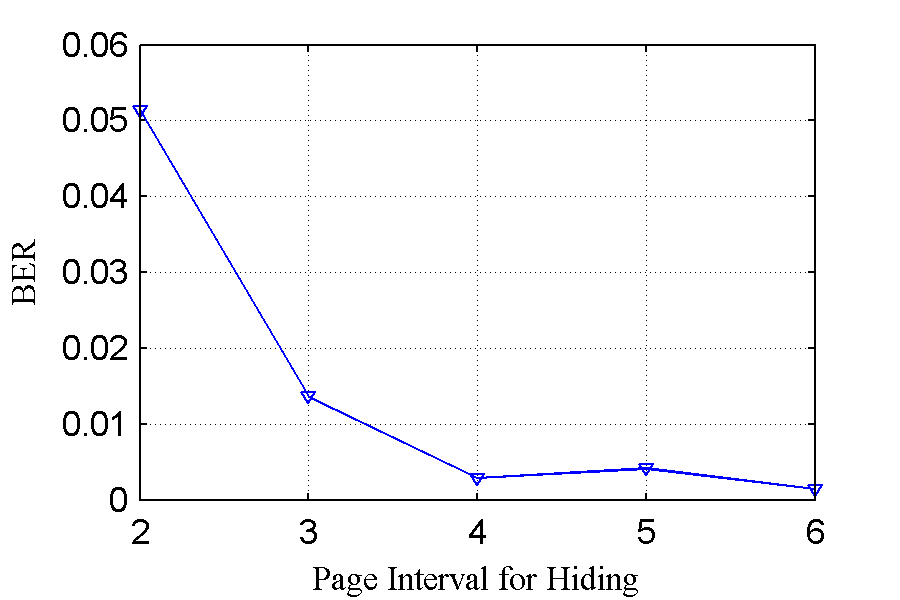
\includegraphics[width=\mywidth]{figs/page_intv.png} 
\caption{Influence of page interval on BER.}
\label{fig:pageintv} 
\vspace{-0.1in}

\end{center} 
\end{figure}

There is also a trade-off between the robustness of the scheme 
and its hiding capacity. When more physical bits are included 
in a group, the capacity decreases. On the other hand, the 
statistical variations among groups will decrease as the group size
increases. Therefore, the BER decreases with an increasing 
group size, as shown in Figure~\ref{fig:groupsize}.  
It is also observed that neighboring pages have a strong influence 
on each other; stressing one page may also cause some stress in a 
neighboring page. To solve this problem, only a subset of pages with
a specific interval $K$ can be used within a block. If $K$ is 4, then only
page 0, page 4, page 8, and so on are used to hide information while
the rest is not used. The influence of this page interval on the BER 
is shown in Figure~\ref{fig:pageintv}. The experimental results suggest
that there is not much benefit to using a group size beyond 128 and a 
page interval beyond 4 for these chips. Figure~\ref{fig:groupsize}
and Figure~\ref{fig:pageintv} were generated from the 2Gbit Micron 
chips, but we found that the group size of 128 and page interval 
of 4 also work well for the 4 Gbit chips.

\begin{figure} 
\begin{center} 
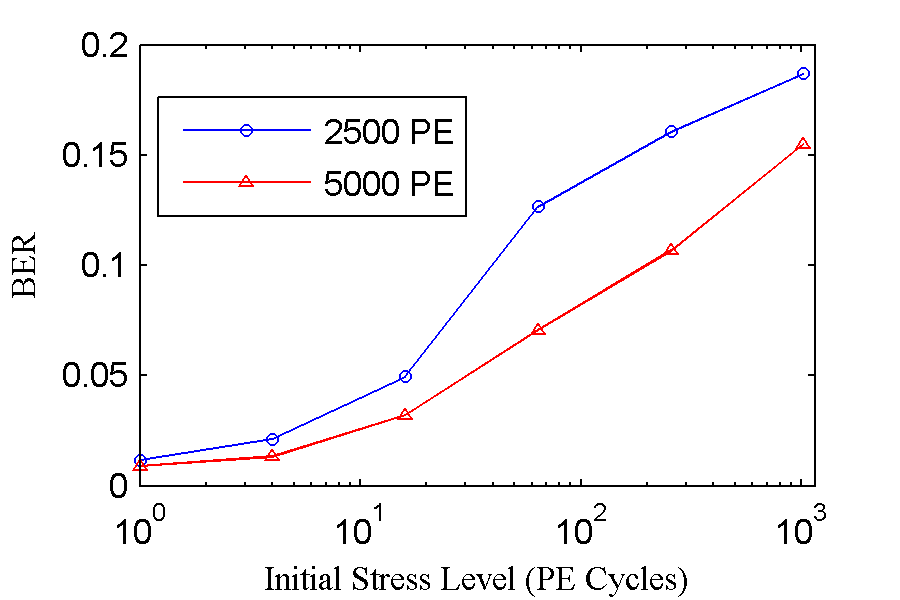
\includegraphics[width=\mywidth]{figs/initialstess.png} 
\caption{Influence of initial stress level on BER.}
\label{fig:initial_stress} 
\vspace{-0.1in}

\end{center} 
\end{figure}

The effectiveness of the method on moderately used Flash chips is also
studied. The influence of the initial stress level before the encoding
process on the BER is shown in Figure~\ref{fig:initial_stress}. 
Here, we aim to simulate the normal usage of the Flash chip. 
So, in each program operation for the initial stress, random data are 
programmed. For example, the BER at the initial stress level of 10 PE 
cycles shows the error rate when bits are hidden after 10 PE cycles of
programming random data.
It can be observed that as the initial stress level increases, 
the BER also increases. 
However, a higher initial stress level can be tolerated by increasing
the stress level in the encoding process.
Note that the error rate is still manageable (less than 10-15\%) even 
after hundreds of normal PE cycles.

\begin{table}
  \begin{center}
    %\begin{scriptsize}
\begin{tabular}{|l|c|c|}
\hline

  & 5,000 Hiding PE & 10,000 Hiding PE \\

\hline
BER after zero retention  & 0.0029 & 0.0021 \\
(1 post PE cycle) & &\\
\hline
BER after 2-day retention &  0.0141 & 0.0035 \\
(3 post PE cycles) & &\\
\hline
BER after 3-day retention & 0.0187 & 0.0045 \\
(5 post PE cycles) & &\\
\hline
BER after over a month & 0.0178 & 0.0031 \\
retention(7 post PE cycles) & &\\
 \hline

\end{tabular}
%\end{scriptsize}


  \end{center}
\vspace{-0.1in}
\caption{Retention characteristics of the hidden message.}
\label{tab:retention}
\vspace{-0.2in}
\end{table}


The retention characteristics of the hiding scheme are shown 
in Table~\ref{tab:retention}. Note that since each decoding 
performs 2 PE cycles, these retention characteristics include
impacts from additional PE cycles in addition to the time
between information hiding and retrieval.
In the first three rows of Table~\ref{tab:retention}, the BER
increases as retention time and post-hiding PE cycles increase. 
In the last row, the BER actually decreases a little compared to the 
third row. 
%Considering that the additional PE cycles reduce the
%intentional biases and increase the BER, we can conclude that the
%retention time has little effect on the BER. 
The results suggest that the retention time has little effect on
the BER.
Intuitively, given that the hiding scheme utilizes cell aging, 
this result is also supported by the fact that a worn-out Flash
memory does not recover greatly even after having been left
unattended for a long time. 


\subsection{Performance}
\label{sec:perf}


In our experiments, when a whole page is used for hiding, 
it takes about 123.6 seconds to perform 5,000
PE cycles of hiding stress on a block, which embeds 2,048 bits of
information in the block. The hiding throughput is around 16.6
bits/second. The upper limit of the throughput can also be calculated using the page
program time and block erase time given in the Flash memory chip
datasheet. The typical page program time is 200 microseconds and
the typical block erase time is 700 microseconds. With 2,048 hidden bits
in 16 pages of a block, the 5,000 PE cycles will take 
$(0.2*16+0.7)*5,000/1,000=19.5$ seconds. The throughput will be about 
105 bits/second. This is the ideal case which does not include 
program data transfers and microcontroller overhead. 
The hiding throughput will also be higher if we use a smaller number of
PE cycles for stressing, or if we use smaller groups. 

%\textbf{TODO: is this presentation reasonable?.}
In order to read the hidden information, one needs to obtain per-bit 
program times using partial programming. The characterization speed depends 
on the number of partial programs, $M$, used in the decoding algorithm. 
For reading hidden bits (decoding), we only need to perform partial programs 
until more than half of the bits flip. 
In our experiment, $M$ for decoding is around 30, 
and it takes around 3.63 seconds to characterize 16 pages, which contain 
2,048 hidden bits. Therefore, the read throughput is about 564 bits/second.  
The read throughput will be higher if the hiding scheme uses a smaller number of
Flash bits to encode each hidden bit.
%When a group has smaller number of cells, the read throughput will be
%higher as we can get more decoded bits out of the same 
%number of Flash bits.
%Still, $M$ depends on the time used for each partial 
%program, $T$. 

For a detailed analysis to detect hidden bits (see \ref{ssec:perbit-analysis}),
one needs to obtain a complete program time distribution with a large $M$. 
In our testbed, it takes 612.6 seconds to characterize a block using 
$M = 1,200$ even if we ignore data transfer from the microcontroller to the host
computer and processing time on the host.
%On average, it takes 2.3 seconds to characterize 4,096 bits in a page.
%If each group has 128 cells, then the 4,096 Flash bits provide 32 bits 
%of hidden information.
%Therefore, the read throughput is about 13.88 bits/second. 
%The typical random read latency is 25 microseconds which is
%quite small compared to 2.3 seconds.
%\textbf{This section needs better numbers.}
%If we use the entire page, which has four times more bits than 
%4,096 bits, obtaining the per-bit program time will take around 
%9.2 seconds. Read throughput will also increase by four times, 
%in this case with a 128 bit group size, to 55.5 bits/second. 
%\textbf{TODO: IS THIS TRUE?} 
A 4Gbit Flash memory chip has 
4,096 blocks, so obtaining the complete program time distribution
of the whole chip will take around 29 days. 
%For decoding,
%it takes around 16.5 hours. 
Higher capacity chips will take even more time to characterize for detection
and decoding. For comparison, simply reading
the digital content from the 4Gbit Flash chip will take approximately 4 minutes. 
Therefore, fully characterizing the entire Flash chip without knowing
where hidden information is located is quite time consuming.

%Suppose one page out of four pages are selected for hiding and each
%group has 128 cells. Then we can hide 1/512 of the
%flash memory chip capacity of raw data. The capacity should be 
%optimized with comprehensive analysis on selected page interval,
%group size and BER which require extra ECC bits.


\subsection{Detectability}

The previous subsection shows that the per-bit program time in Flash memory
can be controlled sufficiently to reliably store hidden 
information. Here, we 
discuss whether an attacker with access to a Flash chip can detect the 
existence of hidden information. In essence, the question is 
whether variations in Flash memory characteristics due to information 
hiding can be distinguished from variations due to normal use. 

The proposed information hiding scheme uses per-bit program time,
which is not visible from the digital content 
in a Flash memory device. Also, the hiding 
operation does not change normal Flash
functions; users can still read, erase, and write Flash memory
in the expected manner.
Therefore, the hidden information cannot be detected from the 
inspection of digital content. Instead, an attacker 
needs to rely on checking the analog properties of the Flash memory.

The following list summarizes the steps that an attacker needs to 
take in order to analyze the analog properties, and in particular, 
the timing properties, of Flash memory.

\begin{enumerate}
\item Check for anomalies in timing of normal Flash operations. 

\item Pick pages/blocks for more detailed analysis.

\item Collect per-bit program time for a selected page.

\item Analyze the per-bit program time distribution of a page.

\item Repeat Steps 2 to 4.

\end{enumerate}

In order to determine whether a Flash chip contains hidden information or not,
an attacker can start by checking the timing of normal Flash operations such as
per-page program time and per-block erase time, which can easily be obtained 
from normal operation. If these operations do 
not show any anomaly -- their timing is within the range of timing 
characteristics for normal use -- then the
attacker needs to obtain and analyze per-bit program time by picking a page for
detailed analysis, collecting per-bit program times through partial programs,
and
then running an analysis. If there is no way to identify suspicious pages and blocks
from normal operations, in the worst case,
the attacker will need to perform the detailed analysis for every single page in Flash 
memory, which will take a long time.
%in a brute-force fashion.

%by brute forcing selection of group size and hiding key in order 
%to determine if a page has hidden data is, and then what that data would be.
%The analog characterization process itself for an entire chip 
%takes a long time (estimated 29 days for the chips used). The cryptoanalysis,
%using group size and hiding key, scales exponentially. If the attacker does
%not know which chip has hidden information on it, characterizing every
%Flash chip that they can reach would be a very slow process.
%Also, an absence of
%this length would be noticed by the hiding party and mitigating steps could be
%taken.
%\textbf{TODO: sort of a weak plan for the hiding party... if that information
%iscritical?}

In the rest of the subsection, we will discuss each step that the attacker
needs
to take and whether the information that is hidden can be 
detected in each step.


\subsubsection{Anomalies in Normal Flash Operations}

%\begin{figure} 
%\begin{center} 
%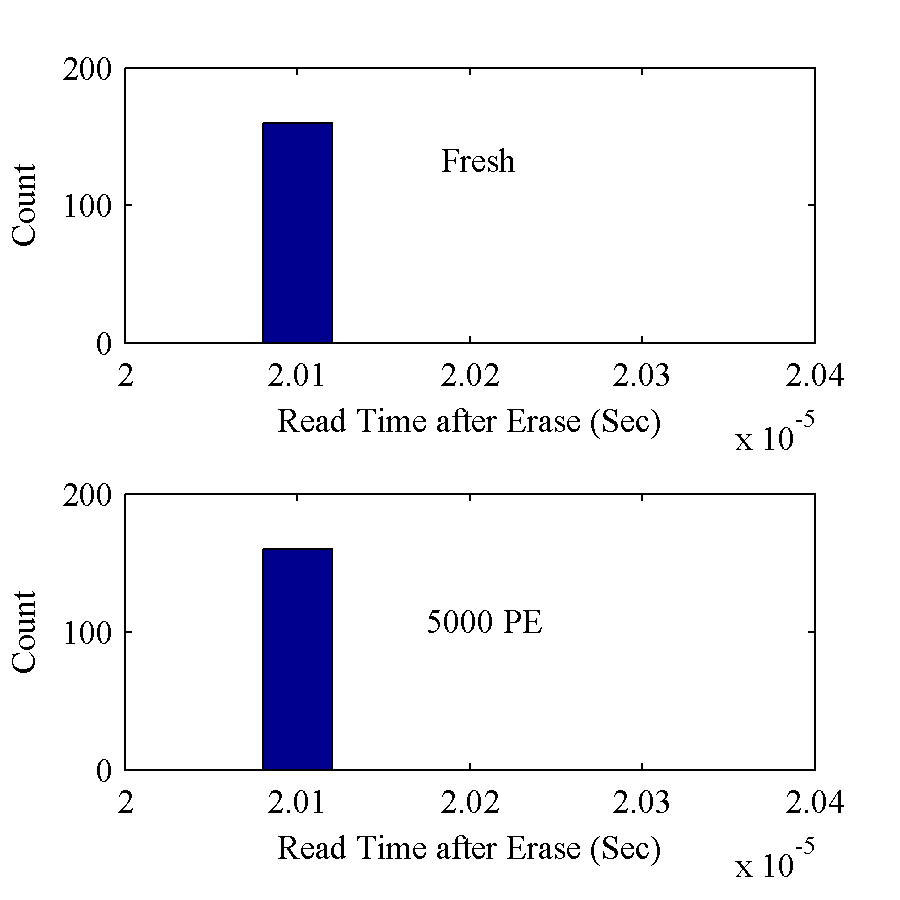
\includegraphics[width=\mywidth]{figs/c6_readtime_aftererase.png} 
%\caption{Read time histogram after block erase. The histogram after page program is similar.}
%\label{fig:rtime_afterprogram} 
%\end{center} 
%\end{figure}

%\begin{figure} 
%\begin{center} 
%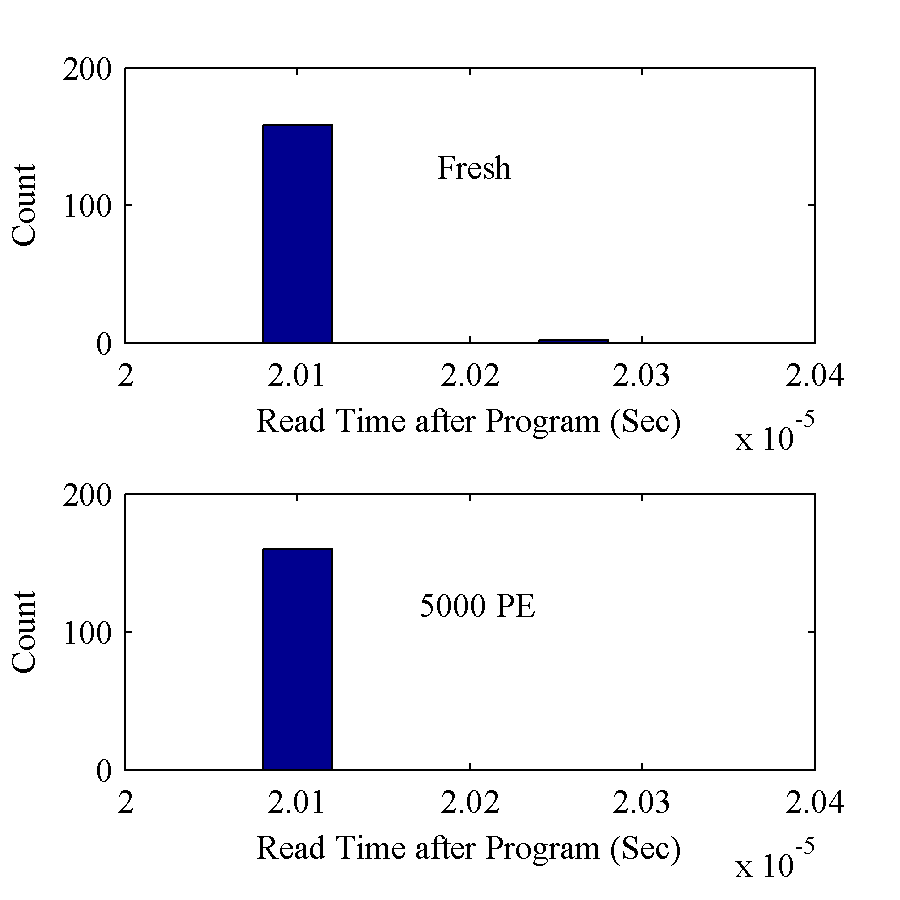
\includegraphics[width=\mywidth]{figs/c6_readtime_afterprogram.png} 
%\caption{Read time histogram after page program.}
%\label{fig:rtime_aftererase} 
%\vspace{-0.1in}
%\end{center} 
%\end{figure}


%\begin{figure} 
%\begin{center} 
%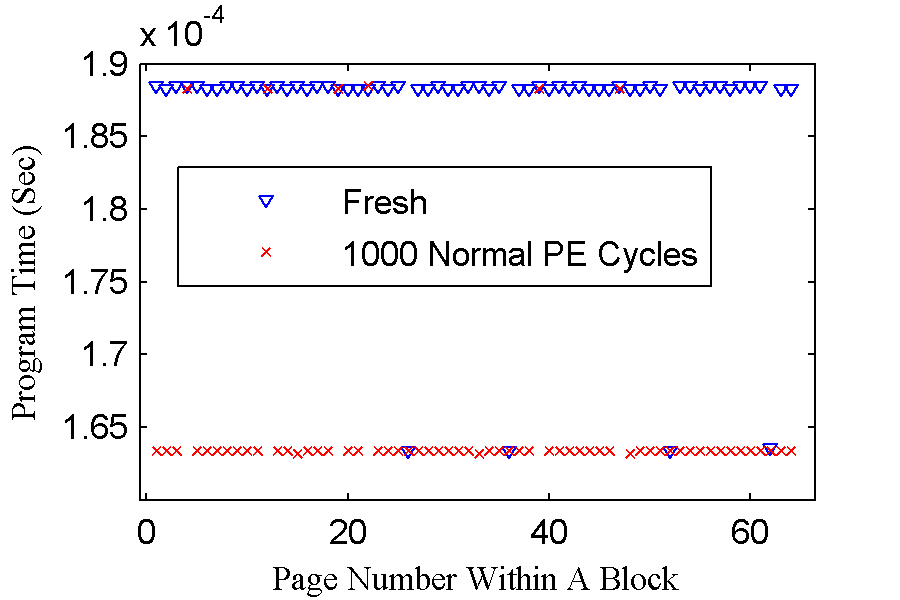
\includegraphics[width=\mywidth]{figs/ptime_normalusage.png} 
%\caption{Program time for pages within a block, normal usage.}
%\label{fig:ptime_normal} 
%\end{center} 
%\end{figure}

%\begin{figure} 
%\begin{center} 
%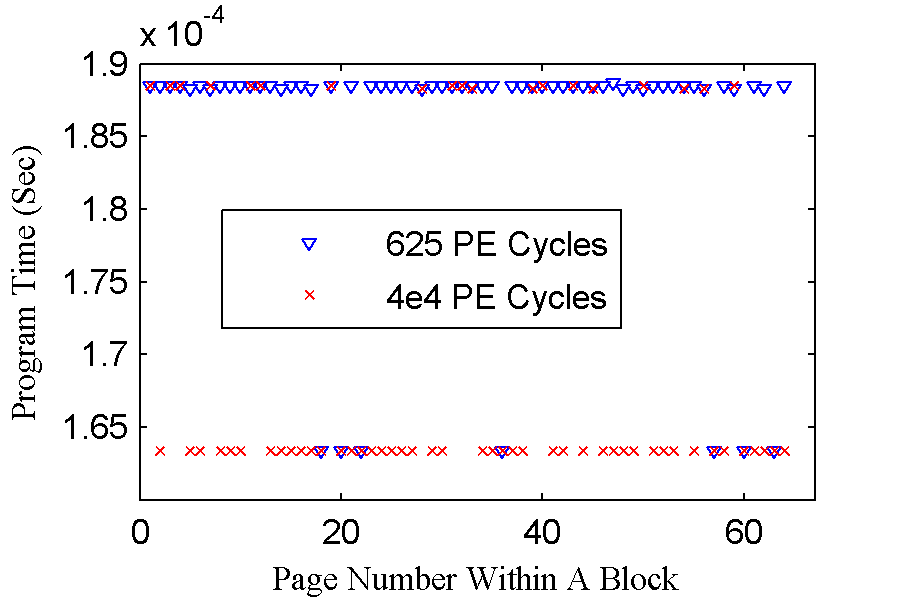
\includegraphics[width=\mywidth]{figs/ptime_hiding.png} 
%\caption{Program time for pages within a block, with hiding.}
%\label{fig:ptime_hide} 
%\vspace{-0.1in}
%\end{center} 
%\end{figure}

%\begin{figure} 
%\begin{center} 
%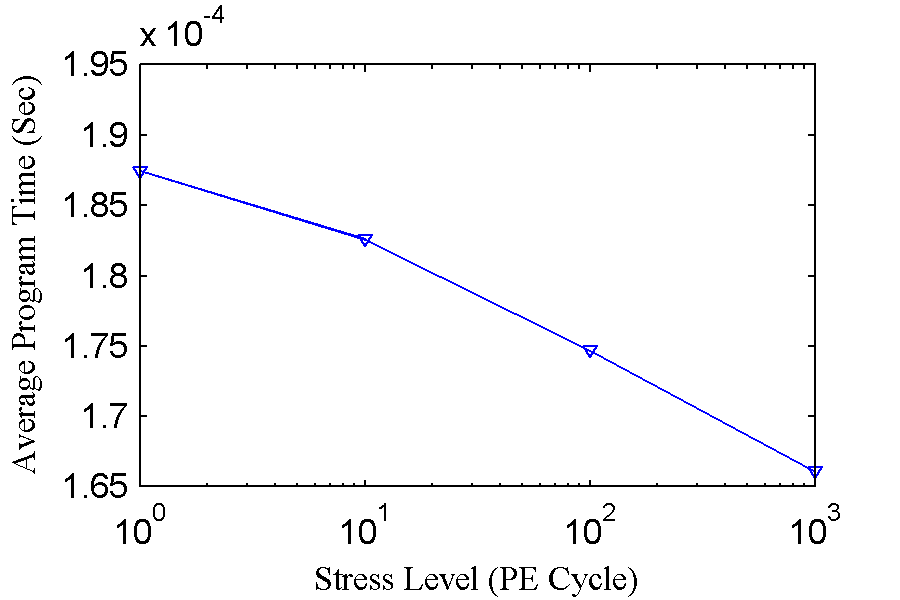
\includegraphics[width=\mywidth]{figs/avgptime_regular.png} 
%\caption{Average page program time for normal usage.}
%\label{fig:avgptime_normal} 
%\vspace{-0.1in}
%\end{center} 
%\end{figure}

%\begin{figure} 
%\begin{center} 
%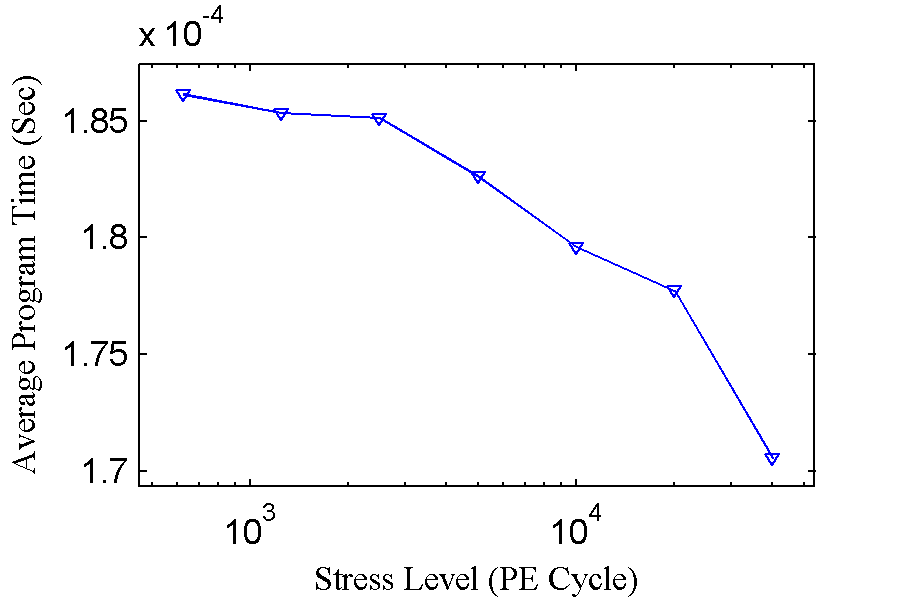
\includegraphics[width=\mywidth]{figs/avgptime_hide.png} 
%\caption{Average page program time for hiding.}
%\label{fig:avgptime_hide} 
%\vspace{-0.1in}
%\end{center} 
%\end{figure}

%\textbf{TODO: need to standardize on "hiding
%PE cycles"; "normal PE cycles". Also "hiding pages".}


Stressing a Flash chip may affect the analog characteristics
of normal memory operations such as page read time, page program time, 
and block erase time. 
If these characteristics change significantly due to our scheme,
an attacker could use that to detect the existence of hidden 
information. Therefore, we first study the impact of information 
hiding and normal Flash use on the page read time, page program time, 
and the block erase time.

Using the Micron 4Gbit chips, we tested six hiding PE cycle counts 
(625, 1,250, 2,500, 5,000, 7,500, and 10,000) and five normal PE 
cycle counts (0, 32, 64, 128, 256) on 4 different chips. On each chip,
we used 20 blocks, 
each containing 64 pages. Because we hide data once every fourth pages, 
only 16 pages within each block are used to hide information.
A normal PE cycle is performed by writing randomly generated data 
to every page in a block, then erasing that block, simulating
wear from normal usage.

To study the impact of information hiding on the page read time,
we measured the time to read pages (after performing
an erase) when they were fresh as well as after 5,000 hiding PE cycles. 
%Figure~\ref{fig:rtime_aftererase}. Read times after a performing a program
%show a similar histogram.
%, and Figure~\ref{fig:rtime_afterprogram}. 
The read times were virtually identical before and after the hiding
stress, showing that the read time would not be a good indicator for 
the existence of hidden information.
%No obvious change caused by stress was visible here, with
%the distributions of fresh page read times and
%pages with hidden information read times coinciding well. 
%This result is expected and coincides with previous literature.

%To the eye it would be nearly impossible to differentiate 
%any existing deviation. 
%\textbf{TODO: I also put data from c3 into the figure directory. Do we want to use that?:}
%A more thorough analysis by support
%vector machine is considered later in the section.
%\textbf{TODO: IF THERE IS A CHANGE:} It appears that pages with hidden 
%information
%tend to have a significant increase in read time. A chip with
%many pages having a high read time could then be considered
%suspicious by an attacker and set aside for further study. 
%It is notable that since chip to chip variation is significant,
%a chip with many high read time pages could also be the
%result of process variation and/or normal usage, and -
%an attacker could only be certain after further analysis.

%figure for page program time within a block 2
%\begin{figure} 
%\begin{center} 
%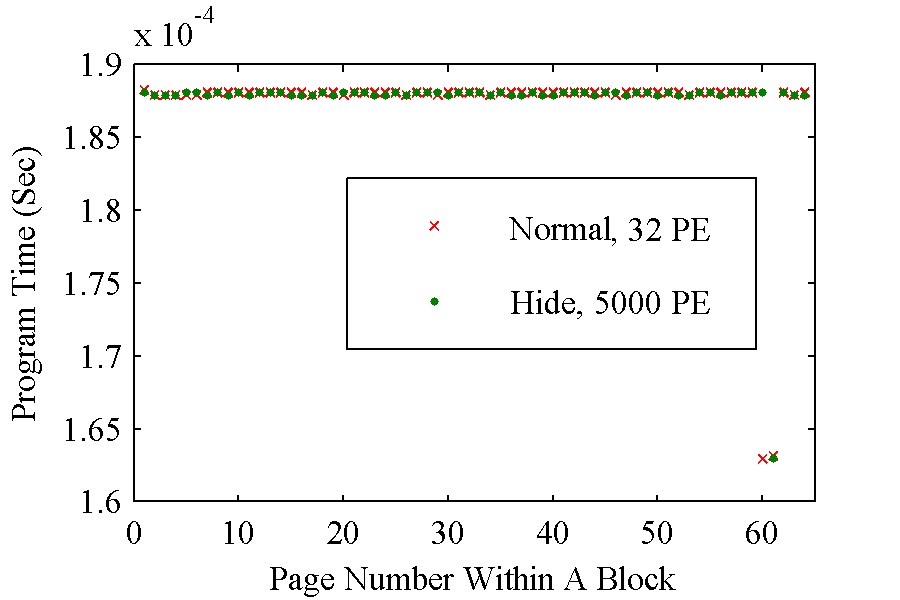
\includegraphics[width=\mywidth]{figs/programtime_5000pe32pe.png} 
%\caption{Program time for 64 pages within a block (not sure whether want to show this one or previous one.}
%\label{fig:ptime_block2} 
%\vspace{-0.1in}
%\end{center} 
%\end{figure}

Figure~\ref{fig:ptime_block1} shows the program times for individual pages in two 
blocks from one chip, one fresh block and the other with hidden information. 
As shown in the figure, 
even though our hiding algorithm only uses every fourth page in a block,
there is no visible pattern in per-page program time.
The figure also shows that
the program time of a page shows distinct values. The distribution between
the distinct program times may change as a page wears out with PE cycles. However, 
we found that the possible program time values for each chip stay the same across 
the range of stress levels in both normal usage and information hiding cases.
%Therefore, each page's program time by itself does not show whether the page has
%hidden information or not. 

%figure for page program time within a block 1
\begin{figure} 
\begin{center} 
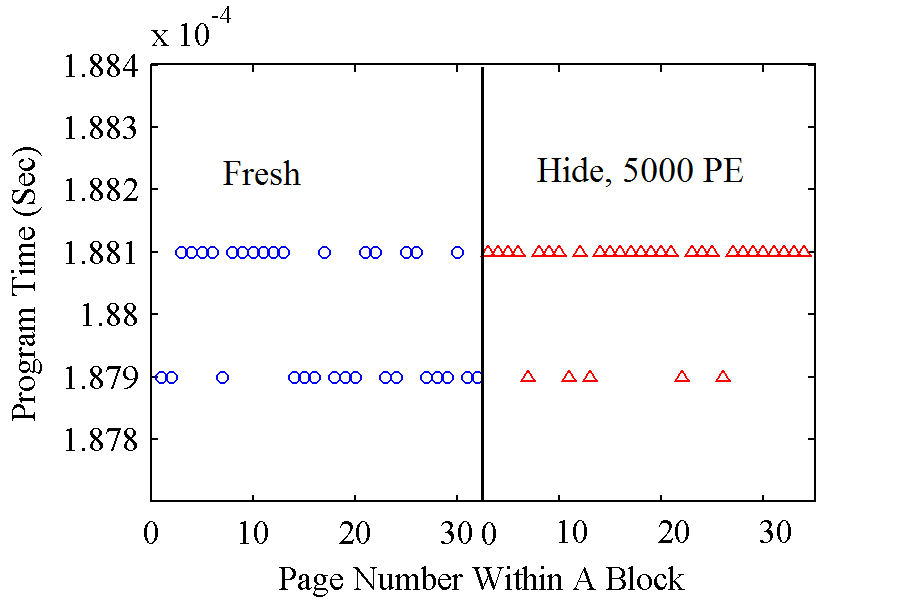
\includegraphics[width=\mywidth]{figs/programtime_block.png} 
\caption{Program time for pages within a block.}
\label{fig:ptime_block1} 
\vspace{-0.1in}

\end{center} 
\end{figure}

%program time histogram
\begin{figure} 
\begin{center} 
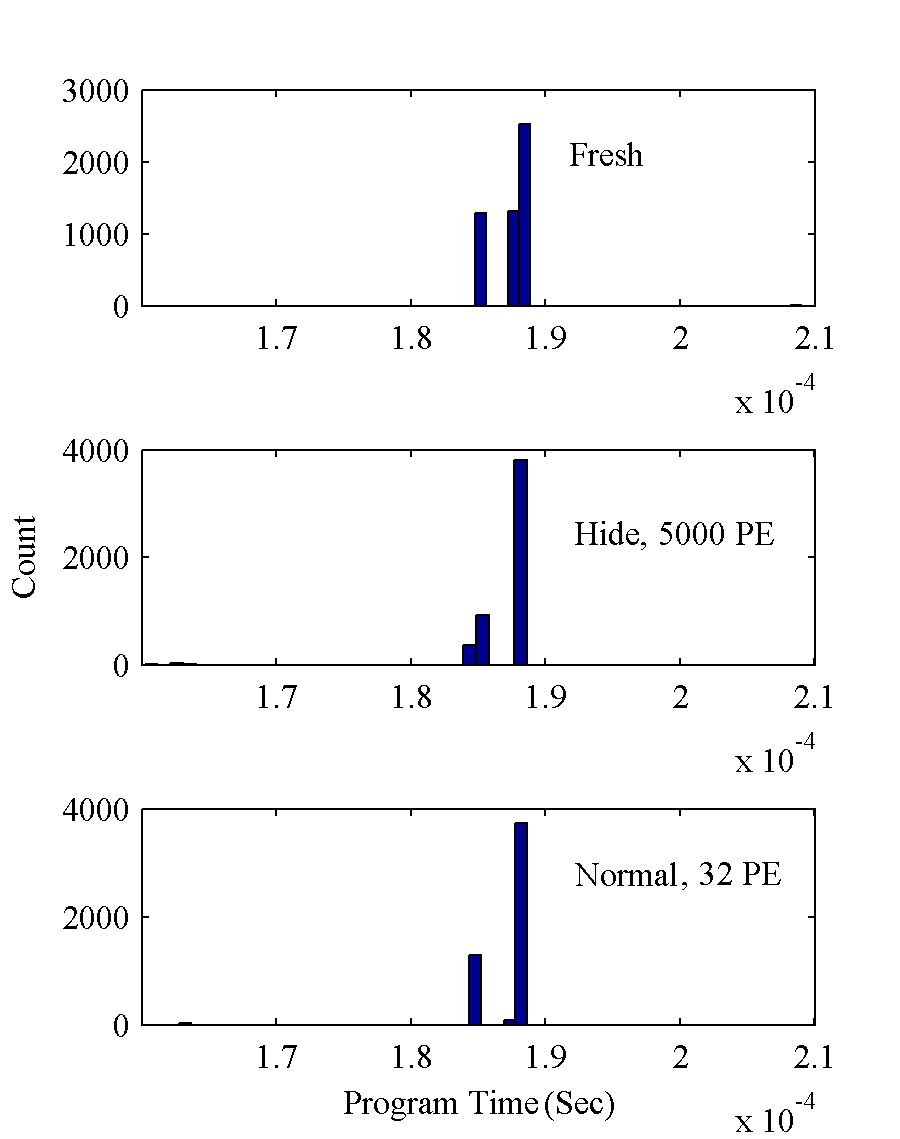
\includegraphics[width=\mywidth]{figs/programtime_hist.png} 
\caption{Program time histogram for three stress levels.}
\label{fig:ptime_histo} 
\vspace{-0.1in}
\end{center} 
\end{figure}


%figure for how the program time change with stress, hide
%\begin{figure} 
%\begin{center} 
%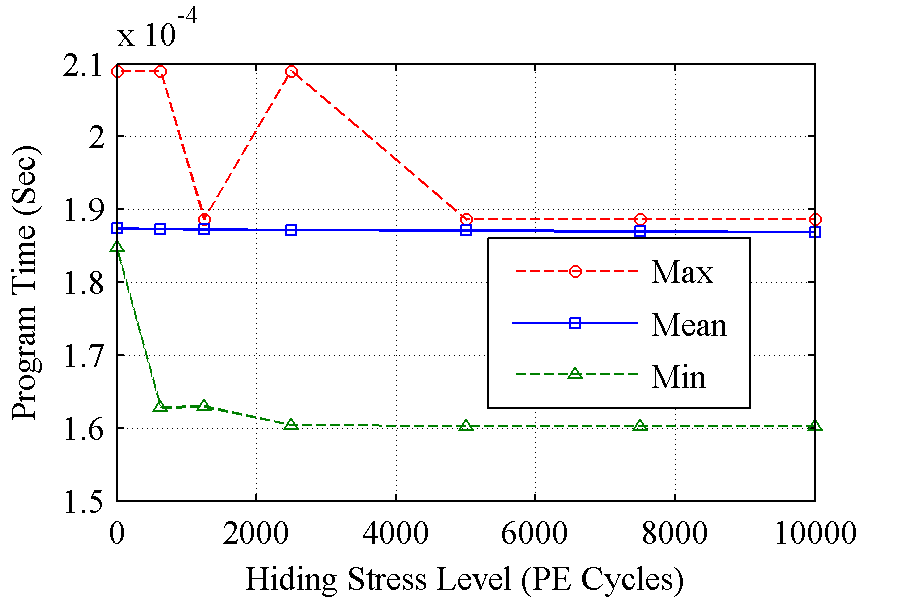
\includegraphics[width=\mywidth]{figs/programtime_hiding.png} 
%\caption{Program time for blocks with hiding.}
%\label{fig:ptime_hide} 
%\vspace{-0.1in}

%\end{center} 
%\end{figure}

%figure for how the program time change with stress, random
%\begin{figure} 
%\begin{center} 
%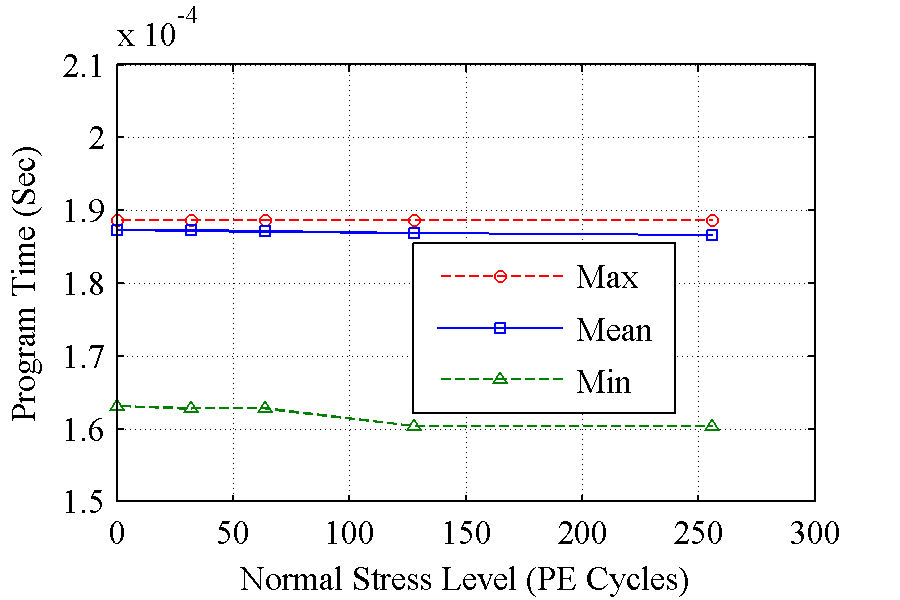
\includegraphics[width=\mywidth]{figs/programtime_normal.png} 
%\caption{Program time for normal blocks.}
%\label{fig:ptime_random} 
%\vspace{-0.1in}

%\end{center} 
%\end{figure}



%\textbf{OLDER DATASET not shown: For the Micron 4G bit chips, 
%we tested 6 chips. For each chip, we tested
%10 blocks for each hide stress level (625, 1250, 2500, 5000, 7500
%and 10,000 PE cycles), 100 fresh blocks, and 5 blocks for each random stress
%level from 1 random PE cycle to 4096 random PE cycles.}
%The histograms for program time and erase
%time are shown in Figure~\ref{fig:ptime_4gchip} and
%Figure~\ref{fig:etime_4gchip}.
Figure~\ref{fig:ptime_histo} shows the program time distributions across
four chips for three different stress levels: fresh, 5,000 hiding PE cycles,
and 32 normal PE cycles. The figure again shows that the program time falls
into a small set of distinct values even though there are more distinct values 
across 4 chips. More importantly, pages with and without hidden information share 
the same set of program time values. 
Also, unlike per-bit program time, the experimental results show that 
the page program time does not change significantly with stress, at least
for the particular 4Gbit chips that we tested.
This is likely due to the fact that the page program time is determined by the
control circuit based on the slowest bit within a page.
Therefore, each page's program time by itself does not show whether the page has
hidden information or not. 

%Therefore, each page's program time by itself does not show whether the page has
%hidden information or not. 

%We can see that for the 4G chips, the page program time is almost 
%not influenced by stress to the eye. We also examine this metric
%later in an SVM. 

%figure for how the erase time change with stress, hide
%\begin{figure} 
%\begin{center} 
%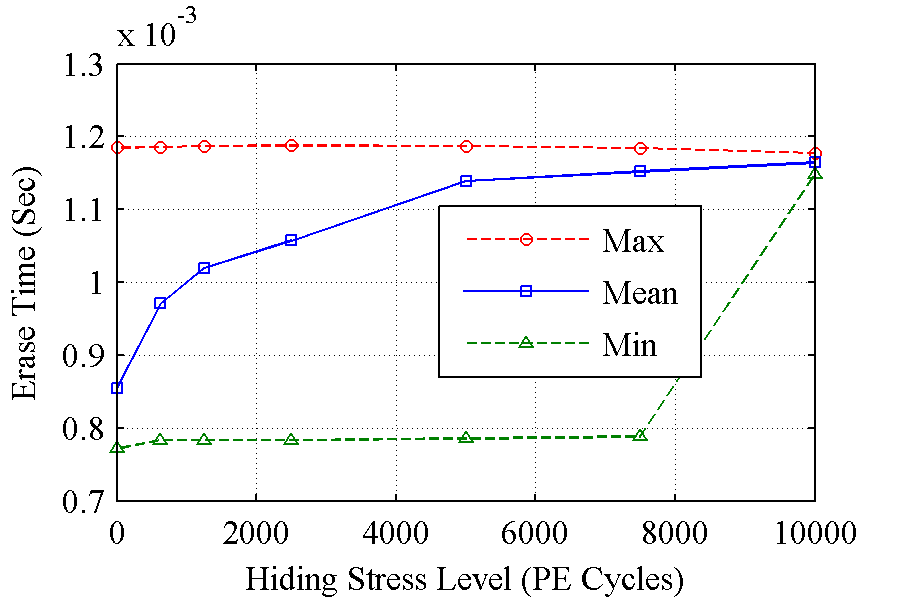
\includegraphics[width=\mywidth]{figs/erasetime_hiding.png} 
%\caption{Erase time for blocks with hiding.}
%\label{fig:etime_hide} 
%\vspace{-0.1in}
%\end{center} 
%\end{figure}

%figure for how the erase time change with stress, random
%\begin{figure} 
%\begin{center} 
%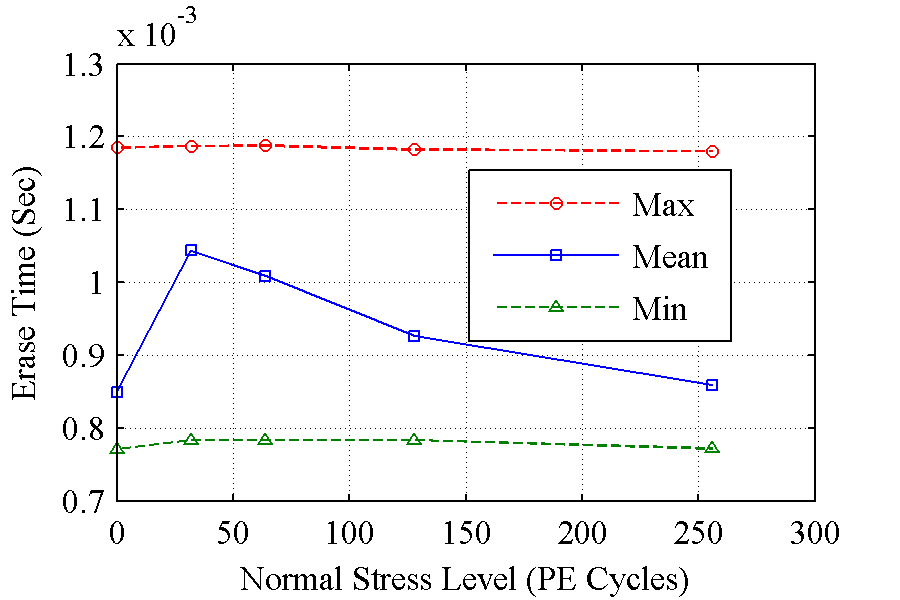
\includegraphics[width=\mywidth]{figs/erasetime_normal.png} 
%\caption{Erase time for normal blocks.}
%\label{fig:etime_random} 
%\vspace{-0.1in}

%\end{center} 
%\end{figure}


%\textbf{TODO 4Gbit erase time data/discussion.}
Figure~\ref{fig:etime_chip1} and Figure~\ref{fig:etime_histo} illustrate the block
erase time distribution within a chip and across 4 chips, respectively.
Similar to the program time, the erase time also falls into a few distinct levels,
which are common across different stress levels. On the other hand,
the figures show that the erase time tends to increase as the stress level
increases. As a result, blocks with hiding stress are more likely to have
a long erase time compared to fresh block without any stress. In that sense,
the erase time may be used to distinguish fresh pages from blocks with hidden bits. 
However, because both normal PE cycles and hiding PE cycles increase
the erase time, it is unclear how to distinguish blocks with hidden information
from blocks with normal PE stress based on the erase time distribution
(see Figure~\ref{fig:etime_histo}). 
We also found that there exist fairly large chip-to-chip variations.
For example, some fresh chips may have over 50\% of blocks that show a long
erase time even without any PE stress. 

%figure for erase time within a chip 1
\begin{figure} 
\begin{center} 
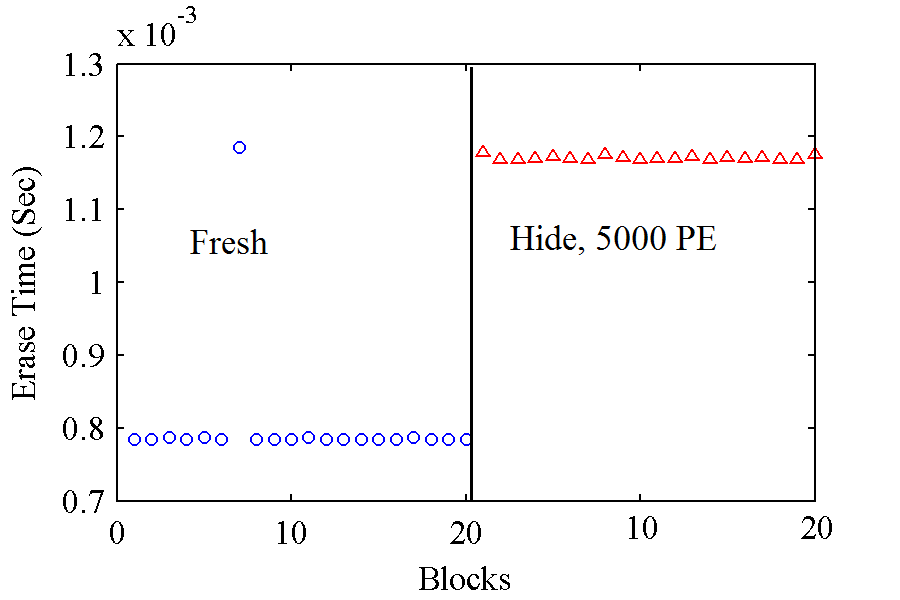
\includegraphics[width=\mywidth]{figs/erasetime_block.png} 
\caption{Erase time for 20 blocks within a chip.}
\label{fig:etime_chip1} 
\vspace{-0.1in}

\end{center} 
\end{figure}

%erase time histogram
\begin{figure} 
\begin{center} 
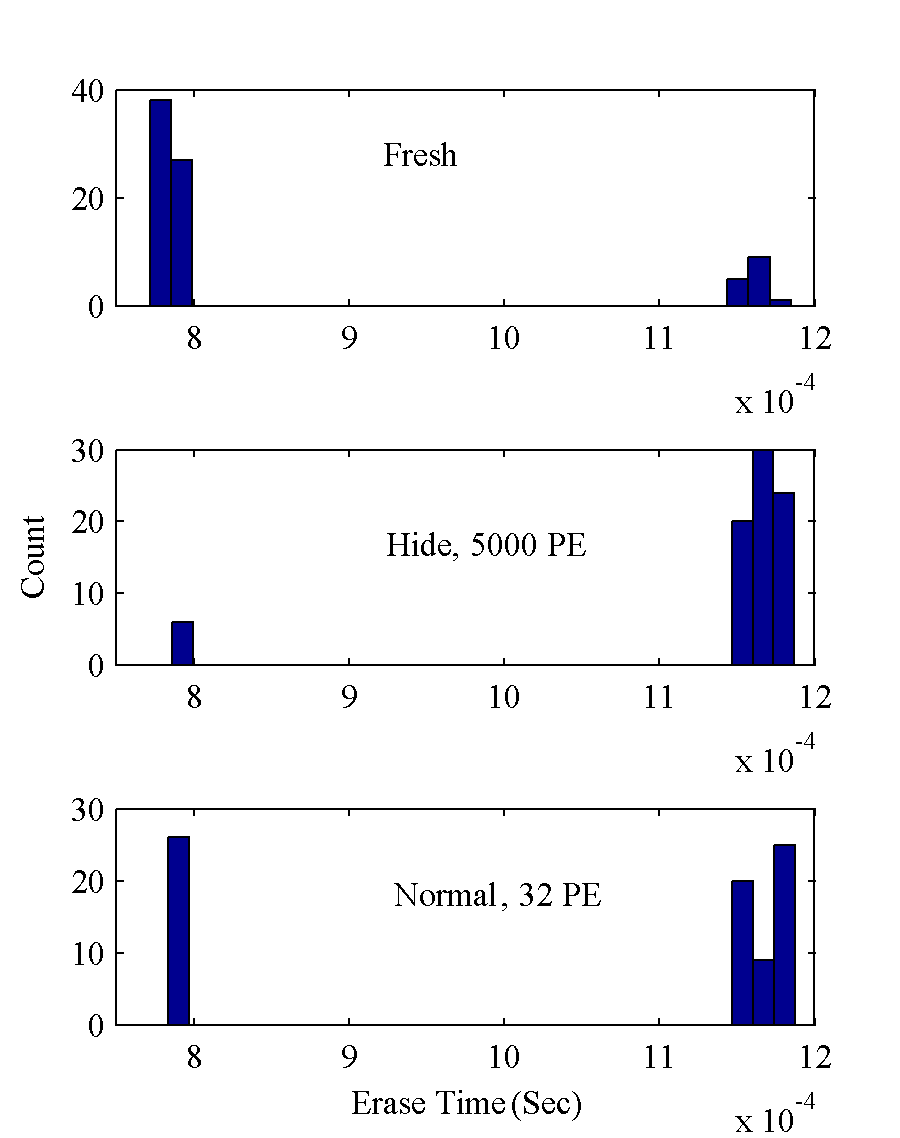
\includegraphics[width=\mywidth]{figs/erasetime_hist.png} 
\caption{Erase time histogram for three stress levels (across 4 chips).}
\label{fig:etime_histo} 
\vspace{-0.1in}

\end{center} 
\end{figure}

%for fresh chips, some chips have few blocks that show larger erase time while
%others have
%a lot of blocks (over 50\%) show bigger erase time. So it is hard to tell
%whether a chip
%with a lot of blocks with bigger erase time has hidden information or not.
%%Further more,
%%even within the same chip, the increase in number of blocks with bigger erase
%%time is
%%negligible under stress level 7500 PE cycles for most of the chips. 
%Since both
%normal blocks
%and blocks with hidden information can have a smaller or bigger block erase
%time, the block
%erase time can not be used for detection based on simple inspection.
 
%The changes of block 
%erase time with hiding and normal stress are shown in Figure~\ref{fig:etime_hiding} 
%and Figure~\ref{fig:etime_normal}, respectively.

%\begin{figure} 
%\begin{center} 
%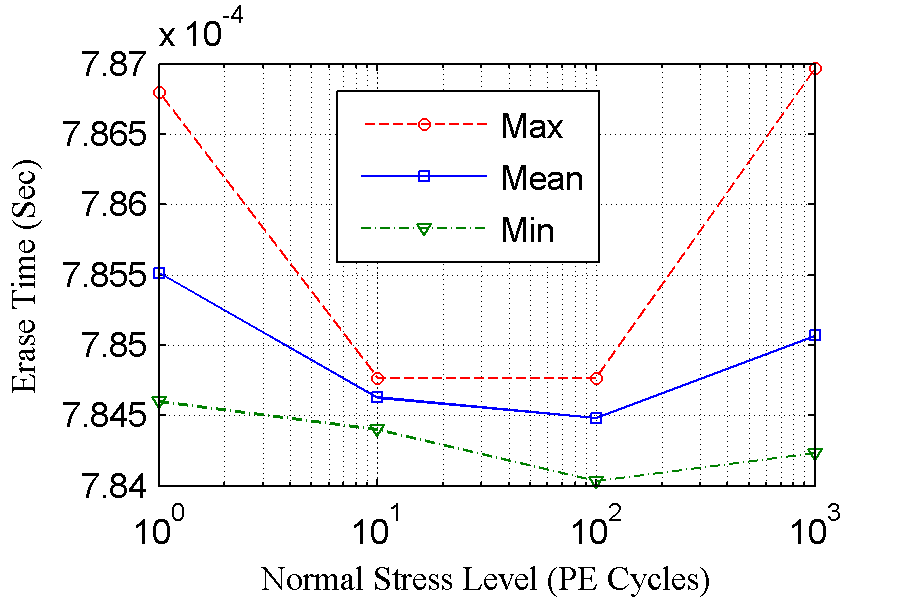
\includegraphics[width=\mywidth]{figs/erase_time_normal.png} 
%\caption{Erase time for normal blocks, 2Gbit chips.}
%\label{fig:etime_normal} 
%\vspace{-0.1in}

%\end{center} 
%\end{figure}

%\begin{figure} 
%\begin{center} 
%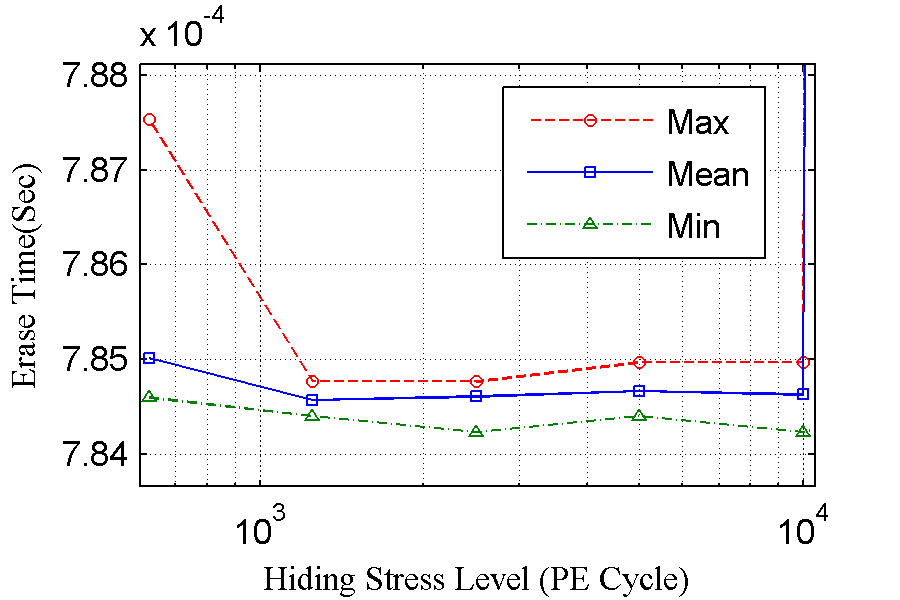
\includegraphics[width=\mywidth]{figs/erase_time_hiding_part.png} 
%\caption{Erase time for blocks with hiding, 2Gbit chips.}
%\label{fig:etime_hiding} 
%\vspace{-0.1in}

%\end{center} 
%\end{figure}

%\textbf{TODO: SVM analysis of page read time, program time, and erase time
%for 4Gbit chips}

The experimental results so far show that there is no obvious pattern in program time 
and erase time distributions to distinguish pages or blocks with hidden information
from pages or block with normal PE stress. 
Yet, it may be possible that there exists a pattern that is difficult to detect
in human eyes. To further study detectability of hidden information based on
normal Flash operations timings, we tried a support vector machine
(SVM) to predict whether a page or a block has hidden information.
A support vector
machine is a machine learning model that is widely used to recognize patterns and
classify data sets. We used libsvm, a popular SVM software package
\cite{libsvm}. 

%The goal of the SVM is to classify a page/block correctly, without
%knowing a priori if a page/block has hidden data or not. 
For the SVM experiments, we constructed multiple data sets using pages/blocks
with hidden information as well as pages/blocks with normal stress, combining
data from one hiding stress level and one normal stress level. We used
two hiding stress levels (2,500 and 5,000 PE cycles) and five normal stress
levels (0, 32, 64, 128, 256 PE cycles), collected from 4 Flash chips.
Then, for each data set, the SVM was trained with data from
3 chips and then tested on data from one remaining chip. 
This construction represents an idealistic scenario for an attacker.
In practice, the attacker will need to consider all possible stress levels for 
both normal uses as well as hiding, which will add more variations.


\begin{figure} 
\begin{center} 
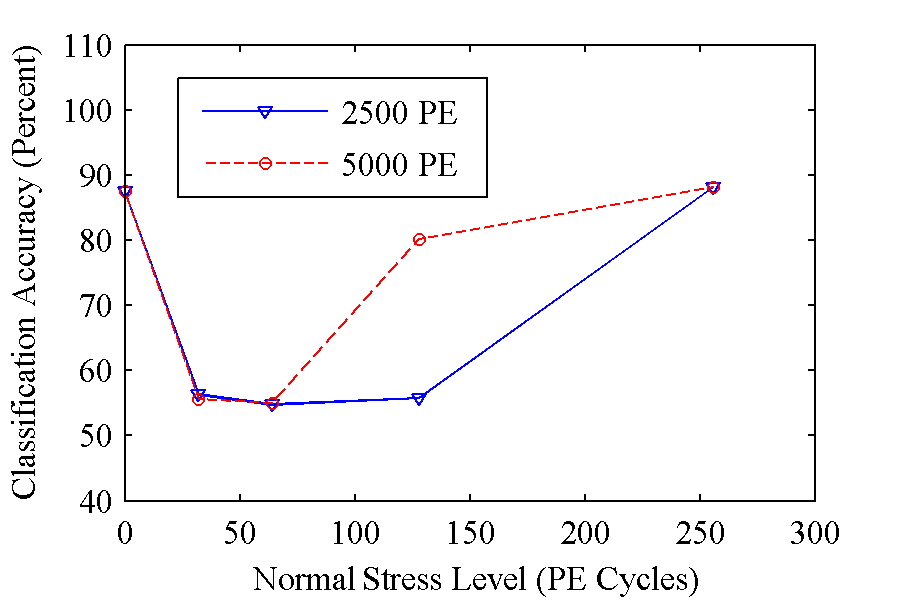
\includegraphics[width=\mywidth]{figs/per_page_svm.png} 
\caption{SVM accuracy for detecting hidden information (per-page analysis).}
\label{fig:page_svm} 
\vspace{-0.1in}

\end{center} 
\end{figure}


\begin{figure} 
\begin{center} 
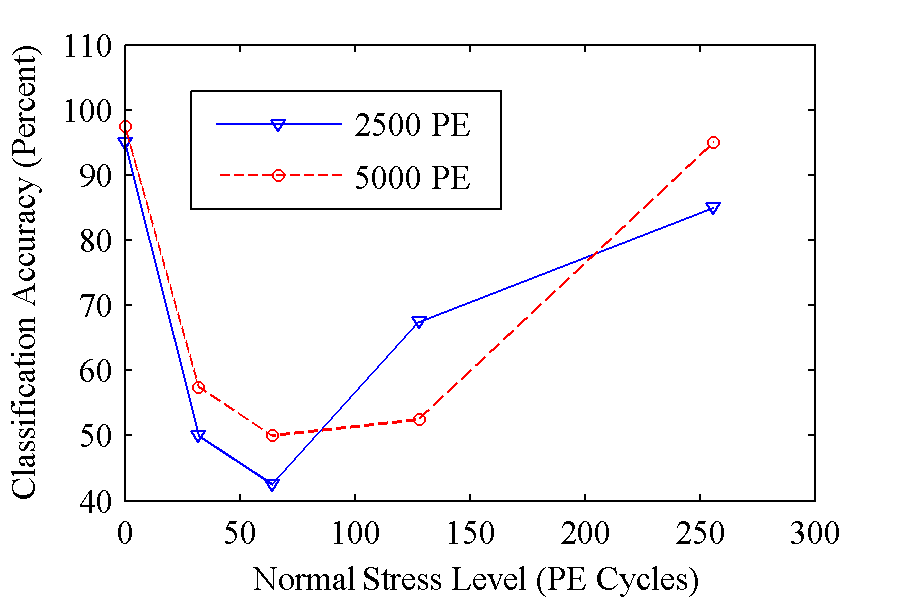
\includegraphics[width=\mywidth]{figs/per_block_svm.png} 
\caption{SVM accuracy for detecting hidden information (per-block analysis).}
\label{fig:block_svm} 
\vspace{-0.1in}

\end{center} 
\end{figure}


Figure~\ref{fig:page_svm} shows the prediction accuracy when the SVM is given
the program time and erase time for each page individually without a notion of
blocks.
The SVM performs relatively well when distinguishing fresh pages and pages
with hiding stress.
However, the accuracy drops significantly when comparing pages with hiding stress
and pages with moderate levels of normal PE stress. In such cases, the accuracy
is not much better than random guesses (50\%).
The SVM performs better again for cases with high normal stress levels beyond 
128 PE cycles because the normal stress exceeds the hiding stress level.
In essence, the results suggest that the SVM can distinguish pages with different
stress levels, but not pages with hiding stress and normal stress.

Figure~\ref{fig:block_svm} shows the accuracy of another SVM construction
where the input vectors were organized by block. In this design, each input 
is a vector of program and erase time pairs for each page within a block, 
allowing the SVM to see a pattern within a block instead of handling each
page separately. The goal of this SVM is to identify blocks with hidden
information. The accuracy of this SVM was similar to that of the 
per-page SVM. The SVM could distinguish more stressed blocks from less stressed
blocks, but not the hiding stress from the normal stress.

While not shown here, we also tested cases where data from all stress levels
were combined together to form a large data set. We found that dealing with
multiple stress levels significantly reduces SVM prediction accuracy for
both the page-granularity analysis and the block-granularity analysis.
The SVM predictions were no better than random guesses.


%\textbf{TODO: the following text corresponds to point 3 in my summary, which notes
%that chip to chip, block to block, page to page, and model to model variation
%is significant too!}


%Although a quick examination of the erase time (with stress level knowledge)
%could indicate a block/chip with hidden data, it is important to note
%that all detected values still fall within the values expected
%from a normally used chip. These values can be highly variable even within
%a chip itself. Blocks and pages in the same chip can show incredible variability
%in program and erase times and in the manner they respond to 
%program and erase stress \textbf{TODO should we cite characterization work?}. 

The experimental results so far show that it is difficult to distinguish pages/blocks
with hiding stress from pages/blocks with normal stress even on one particular
Flash model (Micron 4Gbit). In practice, an adversary will also need to deal with
diversity and variations among multiple Flash manufacturers and models, which will make
detecting hidden bits even more difficult.

In fact, we found that analog characteristics of Flash memory varies significantly
from model to model.
%Although the results suggest that it is more likely that a block with hidden data on it
%would have a higher erase time, this result is only valid for this particular model
%of Flash memory chip. Model to model variation is an important concern for this
%type of analysis. Because there is significant variation
%between models, the behavior of different models can vary greatly and assumptions
%from one model do not necessarily carry over to another.
For example, we tested 2Gbit Flash chips from Micron, which have an identical
specification with the 4Gbit chips except for the capacity. 
%Compared to the Micron 4Gbit chips, their 
%datasheets indicate identical specs but for one difference: the 2Gbit chips have feature 
%set E (fifth generation) while the 4Gbit chips have feature set D 
%(fourth generation), as shown in the product part number. 
Surprisingly, the 2GBit chips, although only a generation apart from
the 4Gbit chips, showed a markedly different behavior compared to the 4Gbit chips. 
For 2Gbit chips, the PE stress had little impact on block erase time
while noticeably changing page program time. In essence, the 2Gbit chips showed
the opposite type of behavior as the 4Gbit chips where the erase time shows
a significant shift. In both cases, we still found that it is difficult to distinguish
the impact of hiding stress from that of normal stress. 

%Almost no difference was seen in the erase times of blocks
%with hidden data and blocks stressed normally, but 
%significant variation did exist in the distributions of program times 
%of hidden vs. normally used pages. In essence, the 2Gbit chips showed
%the opposite type of behavior as the 4Gbit chips.

The significant variations across Flash models imply that an attacker will
need to build and train an SVM model for each Flash chip model in order to use the SVM
for determining the existence of hidden data on a particular chip. 
%The significance of this finding is that for an attacker to
%use normal Flash operation times to 
%determine the existence of hidden data on a particular chip,
%an SVM model would 
%have to be built and characterized for every type of Flash
%chip in which they are interested. 
Obviously, this would require a significant investment on the part of the attacker.
Even then, as we have shown above, there is no guarantee that an SVM
model using normal Flash operations 
will be able to determine the existence of hidden data with a high
probability.

%One thing to note is that for different generations of chips, even two products 
%from the same manufacturer and with very similar specifications, the normal page 
%program time and block erase time can show very different behaviors 
%with stress. 

% MICRON 2Gbit test conditions -- leave them out here?
%For the Micron 2Gbit chips, we tested 5 blocks, each having 64 pages,
%for each hiding stress level and normal PE cycles (writing random data).
%We used 625, 1250, 2500, 5000 and 10000 hiding PE cycles, and 1, 10, 100, 
%and 1000 normal usage.

%\textbf{TODO this page program time section is from the 2Gbit chip data
%and lifted from what we had before.}
%Second, for page program times, we found that a program time of a page
%always shows one of two distinct values for all stress levels in
%normal usage and hiding processes.
%As the stress level (the number of PE cycles) 
%increases in both normal usage and hiding, the number of pages
%with a longer program time decreases and the number of pages with
%a shorter program time increases. Figure~\ref{fig:ptime_normal}
%shows the page program times for pages in two blocks with normal
%stress and Figure~\ref{fig:ptime_hide} shows the page program
%time for pages in another two blocks with hidden information. From the two
%figures, we can see that the two distinct values for page program time
%are the same across the stress levels in both normal
%usage and information hiding. We can also see that even though a
%fixed page interval is used to hide information within a block,
%this does not create a regular pattern of page program times for
%pages within a manipulated block.

%To measure the increase in the number of pages with a shorter page
%program time when the stress level is increased, the average page
%program time is plotted. Figure~\ref{fig:avgptime_normal} shows
%the average page program time in the normal usage situation and
%Figure~\ref{fig:avgptime_hide} shows the average page program
%time with hidden information. The two figures show that the
%stress level has a bigger influence on the page program time in
%the regular usage situation than in the hiding situation.
%Therefore, even though the blocks with hidden information
%experience more PE cycles, they are indistinguishable from
%moderately used blocks under normal usage from the perspective of 
%page program time.

%At the circuit level, this result is expected because the
%page program time is determined by the few slowest programming
%bits in a page. In normal usage, almost every bit is
%programmed to 0 in about a half of PE cycles. In the hiding process, nearly
%half of the bits are only programmed to 1. Therefore, the
%programming speed of the slowest programming bits in regular
%usage should increase faster than the slowest programming bits
%used to hide information. Note that the range of the average program
%times for the pages used to hide information (1.70 to 1.86 s) is completely
%contained in the range of program times for pages used normally (1.66 to 1.88
%s).



%\textbf{TODO: this discussion is for 2Gbit chips.}
%The block erase time for blocks under normal usage and blocks
%used for hiding information are shown in
%Figure~\ref{fig:etime_normal} and Figure~\ref{fig:etime_hiding},
%respectively. 
%We can see
%that for hiding stresses up to 10,000 PE cycles, the block erase
%time for manipulated blocks is indistinguishable from blocks
%under normal usage. 
%This result suggests that the hiding scheme with 10,000 PE cycles
%or less cannot be detected by looking at the erase time distribution.

%%But for a hiding stress of 20,000 PE cycles and
%%40,000 PE cycles, there is a noticeable increase in block erase time.
%%For 20,000 PE cycles, some manipulated blocks are
%%indistinguishable, as seen from the minimum value of the block
%%erase times. For 40,000 PE cycles, most of the manipulated blocks
%%have a higher block erase time than moderately used blocks.
%%Yet, a high PE stress beyond 10,000 cycles should 
%%only be used when the adversary is not explicitly checking the 
%%erase time.

%\begin{figure} 
%\begin{center} 
%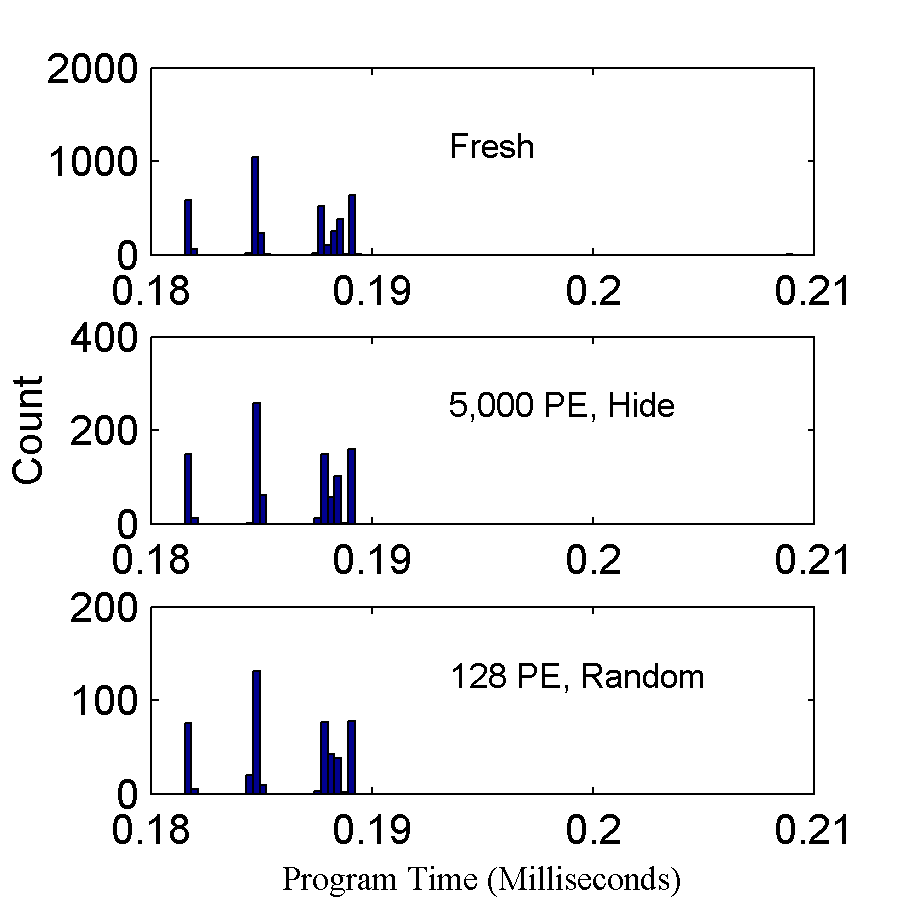
\includegraphics[width=\mywidth]{figs/programtime_histo.png} 
%\caption{Program time distribution for Micron 4G chip.}
%\label{fig:ptime_4gchip} 
%\vspace{-0.1in}

%\end{center} 
%\end{figure}

%\begin{figure} 
%\begin{center} 
%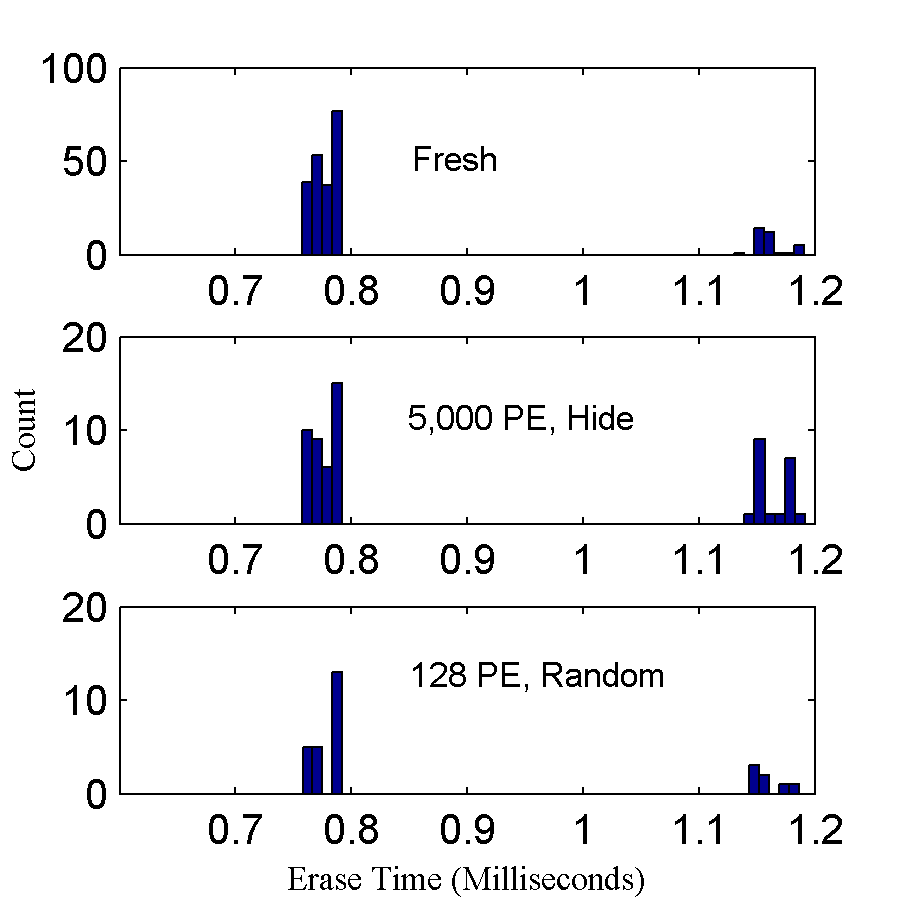
\includegraphics[width=\mywidth]{figs/erasetime_histo.png} 
%\caption{Erase time distribution for Micron 4G chip.}
%\label{fig:etime_4gchip} 
%\vspace{-0.1in}

%\end{center} 
%\end{figure}

\subsubsection{Page Selection and Per-Bit Program Time Collection}

%\textbf{TODO: NOTE: This section largely unchanged.}


%Determining which pages have hidden data on them by inspection of their read,
%program, and erase times is difficult because hidden pages have values that 
%fit within
%the noise of normally used pages. Our experiments showed that a hiding PE of
%5,000 cycles was low enough to remain hidden in the noise of the normally used
%pages, allowing them to remain indistinguishable from fresh pages or moderately
%used pages.

%If a higher hiding PE cycle count is used, then it may become obvious which pages have been
%used to hide data. In this case, other pages (up to the entire chip) could be
%stressed to a similar level, thereby cloaking the hidden page again. This would
%slow down the hiding process, however.

% WE NEED TO GIVE MORE DETAILED RESULTS, NOT JUST A CLAIM.
%As we have seen, there is no certainty that blocks with hidden information 
%can be determined from 
The study of normal Flash operations shows that an adversary cannot simply determine
whether a Flash chip has hidden information or not based on measurements of normal 
Flash operation times. In essence, the hiding stress cannot be effectively distinguished 
from normal PE stress. As a result, an attacker needs to perform a more detailed
analysis on per-bit program times in an attempt 
to determine the existence of hidden data, which we will discuss next.

%Without a fast and effective way to identify potential pages or blocks with 
%hidden information, an adversary
To perform the detailed analysis of each page, the attacker will have to
characterize each page. However, characterizing per-bit program time for every page is 
quite a time-consuming process. As discussed in 
Section~\ref{sec:perf}, a 4 Gbit Flash memory chip requires around 29 
days to characterize. For larger chips, which are common today, the per-bit characterization
will take even longer. 

%While an analysis of normal Flash operation times may not provide enough certainty
%in the detection of hidden information, it may be able to provide candidate locations 
%for an attacker to examine more closely. 
To avoid expensive characterization of every page, an attacker may be able to use
normal Flash operation times to select candidate pages for the detailed analysis.
For example, for the 4Gbit Micron chips, an attacker 
may consider blocks with a higher erase time to be more likely to have hidden information.
%An attacker could start by selectively characterizing these blocks at
%the per-bit program time level. We note that it is possible 
%that blocks with hiding stress can be disguised 
%by stressing other blocks on the chip with a moderate number of normal PE 
%cycles.
However, the study in the previous subsection suggests that pages and blocks with hiding
stress can be hidden by stressing other blocks on the chip with a moderate number of normal PE 
cycles. 
%Some blocks with hidden information will not show up with a 
%higher erase time and could be missed. 

%The only way to be 
%certain would be to collect per-bit program times for every page.

%Note that after per-bit program time collection, there remains the need to crack the
%hiding key to discover the existence of any hidden information.

\subsubsection{Per-Bit Program Time Analysis}
\label{ssec:perbit-analysis}

%\begin{figure} 
%\begin{center} 
%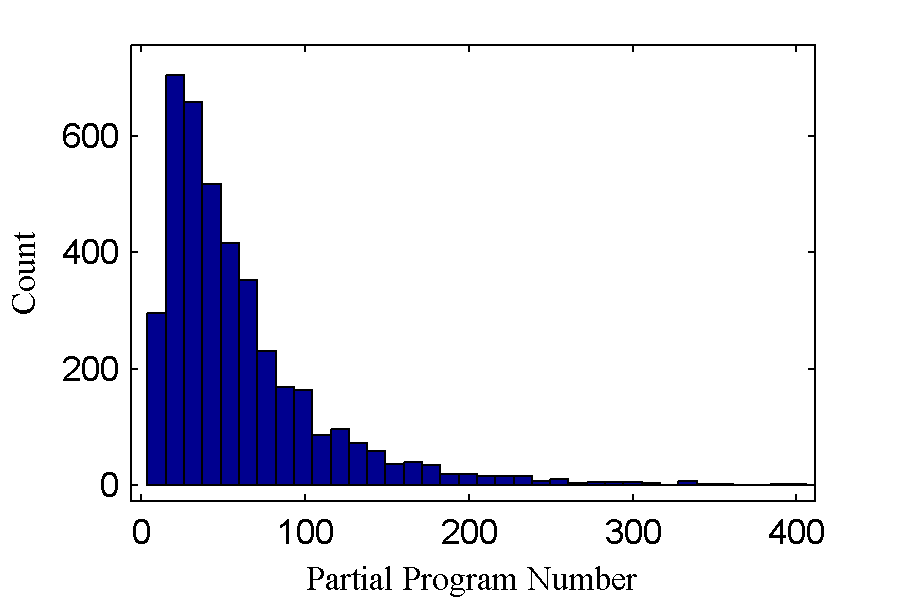
\includegraphics[width=\mywidth]{figs/10rpe_histo_normalusage.png} 
%\includegraphics[width=3.0in]{figs/eval_performance_diff_context.pdf} 
%\caption{Partial program time distribution for bits in a page
% with 10 normal PE cycles only.}
%\label{fig:hist_10penormal} 
%\vspace{-0.1in}

%\end{center} 
%\end{figure}

%\begin{figure} 
%\begin{center} 
%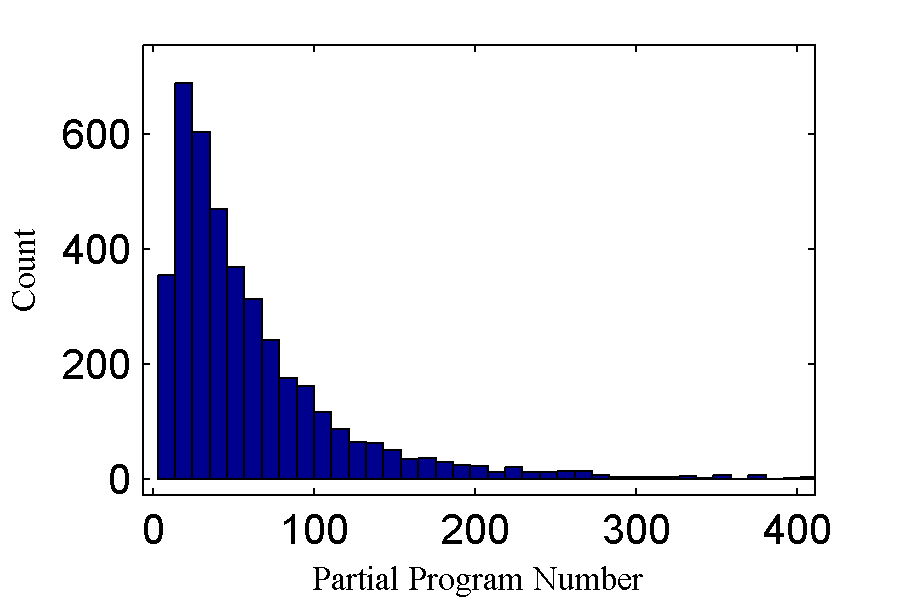
\includegraphics[width=\mywidth]{figs/100rpe_histo_normalusage.png} 
%\includegraphics[width=3.0in]{figs/eval_performance_diff_context.pdf} 
%\caption{Partial program time distribution for 
%bits in a page with 100 normal PE cycles only.}
%\label{fig:hist_100penormal} 
%\vspace{-0.1in}

%\end{center} 
%\end{figure}

\begin{figure} 
\begin{center} 
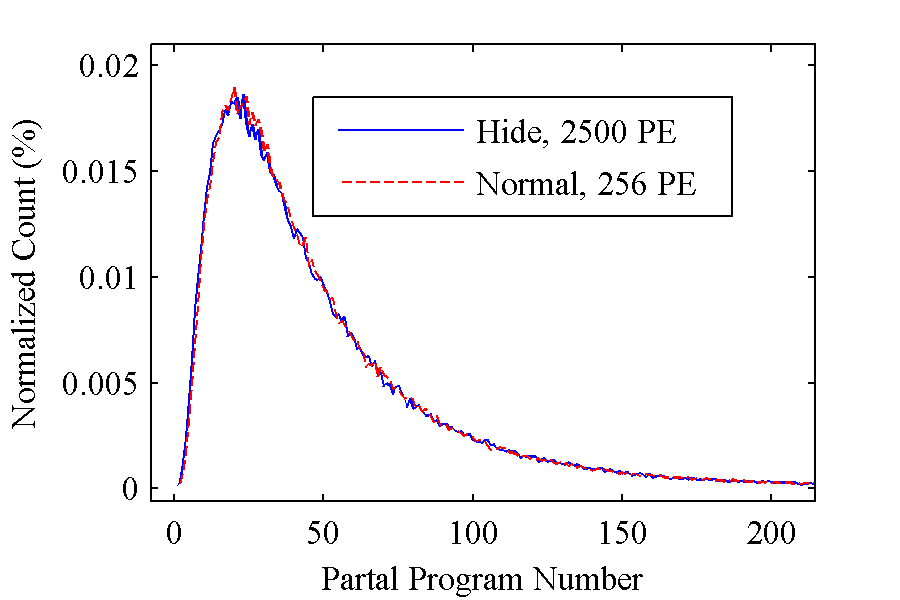
\includegraphics[width=\mywidth]{figs/histo_compare.png} 
%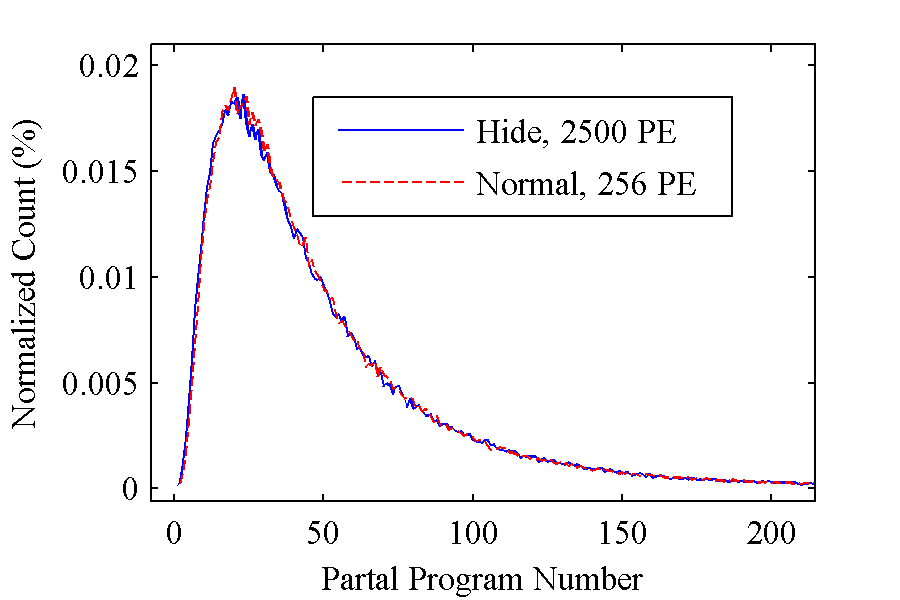
\includegraphics[width=3.0in]{figs/histo_compare.png} 
\caption{Partial program number distribution curve averaged over 5 blocks.}
\label{fig:histo_comp} 
\vspace{-0.1in}

\end{center} 
\end{figure}

A more detailed detectability analysis involves analyzing the partial program
time distribution for bits within a page. In normal usage, the bits are
programmed 0s and 1s randomly over time. In the hiding scheme, some bits are
always programmed 0s and others are always programmed 1s. However, the hiding
scheme does not cause an obvious bimodal distribution due to large intrinsic
variations of bits in a page. Figure~\ref{fig:histo_comp} shows the partial
program time distribution averaged over 5 blocks. It can be seen that they are
very similar to each other.

To statistically analyze the distributions, we turned to support vector
machines again. To train an SVM for the per-bit analysis,
we prepared pages across 2 different hiding PE stress levels (2,500 and 5,000)
and 8 different normal wear stress levels (32, 64, 128, 256, 512, 1,024, 2,048, and 
4,096 PE cycles). We used 5 blocks on each chip, 16 pages per block, for a total
of 80 pages per chip, at each stress level; i.e. on one
chip, there are 80 pages with a hidden message stressed at 2,500 hiding PE
cycles, 80 pages with a hidden message stressed at 5,000 hiding PE cycles, 80
pages without hidden data stressed 32 normal PE cycles, and so on. We
characterized pages across 15 different chips. Each page represents a data
point in the SVM. The SVM had access to the complete raw data for each page: the
vector representing a page and an entry for each bit, with the entry's value as
the partial program time.

We then grouped the data from all chips into multiple sets, combining one hiding 
stress level and one normal stress level.
For example, one data set comprises the hidden data with 2,500 hiding PE
cycles and the data with 128 normal PE cycles, another data set used 5,000 PE
hidden data and 4,096 normal PE cycles, and so on, with a data set for each
combination of hiding and normal PE cycles.

\begin{figure} 
\begin{center} 
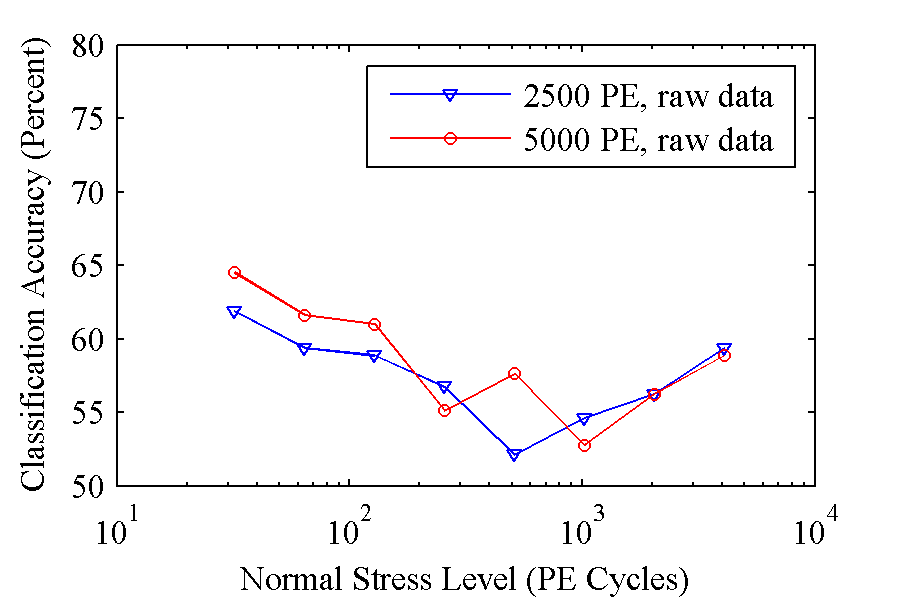
\includegraphics[width=\mywidth]{figs/svm_rawdata.png} 
\caption{SVM accuracy for detecting pages with hidden information (using raw data).}
\label{fig:svm_acc1} 
\vspace{-0.1in}
\end{center} 
\end{figure}

\begin{figure} 
\begin{center} 
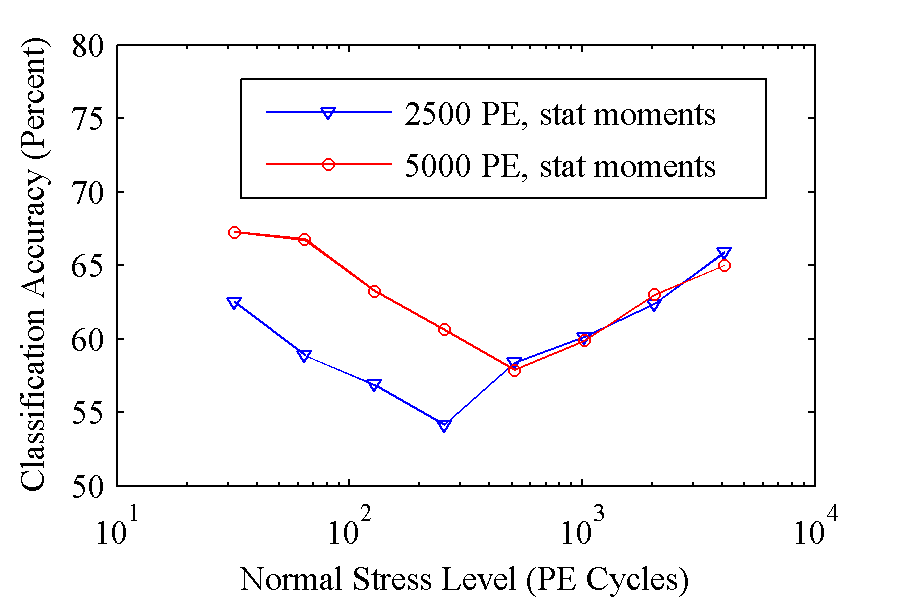
\includegraphics[width=\mywidth]{figs/svm_stat_moments.png} 
\caption{SVM accuracy for detecting pages with hidden information (using statistical moments).}
\label{fig:svm_acc2} 
\vspace{-0.1in}
\end{center} 
\end{figure}

For each data set we labeled the hidden pages and non-hidden pages
appropriately, trained the SVM with data from chips 1-10, and then used the
resulting SVM to predict data from chips 11-15. Overall prediction accuracy of
the SVM on test data from chips 11-15 is shown in Figure~\ref{fig:svm_acc1} 
and Figure~\ref{fig:svm_acc2}.

Each data set is represented by a point in Figure~\ref{fig:svm_acc1}. Normal
PE stress level is shown on the X-axis. The data sets sharing 2,500 hiding
PE
stress are connected by a solid line; the data sets sharing 5,000 hiding
PE stress are connected by a dashed line. Accuracy is shown on the Y-axis.

Overall accuracy is slightly better than random (50\%) for all data sets, with
increased accuracy near the extremes of normal PE stress cycles. This matches
the expectation that a given page with a certain hiding PE stress level
looks similar to a page with a certain normal PE stress level. The further
the normal PE stress level varies from the matching hidden PE stress level,
accuracy should increase.

The data sets in
Figure~\ref{fig:svm_acc2} show the SVM accuracy using a different representation
for page characteristics. Instead of using the partial program 
count for every single bit in a page,
a page was summarized by several statistical parameters:
minimum, maximum, average, variance, skew, and kurtosis. We can see that
prediction accuracy is similar to the SVM using the raw bit-level data.
%, and
%that the extremes of normal PE stress also show an increase in accuracy.

\begin{figure} 
\begin{center} 
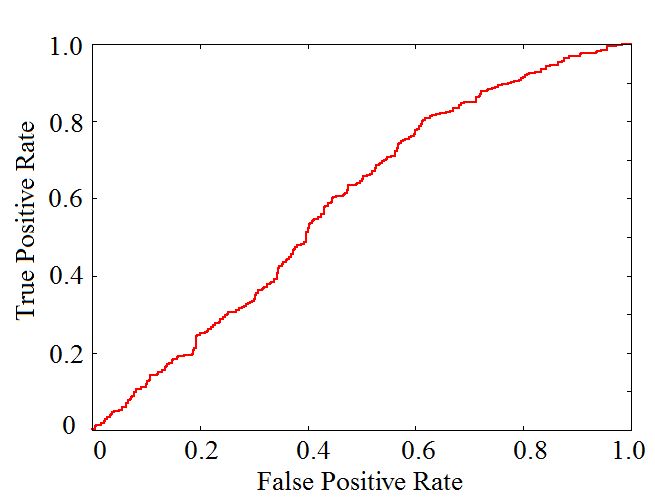
\includegraphics[width=\mywidth]{figs/roc2500128.png} 
\caption{Receiver operating characteristic curve for data set including 2500
hiding PE and 128 normal PE stresses.}
% need to increase figure font size
\label{fig:roc2500-128} 
\vspace{-0.1in}

\end{center} 
\end{figure}

Figure~\ref{fig:roc2500-128} shows a more detailed analysis of the SVM accuracy
using the data set for 2,500 hiding and 128 normal stresses levels.
The receiver operating characteristic (ROC) curve plots the true
positive rate versus the false positive rate, and gives an indication of how
accurate the SVM prediction is, for a given false positive rate. 
The graph shows that the SVM prediction cannot
achieve a high true positive rate without incurring a large percentage of false
positives.
%, indicating that the SVM has a difficult time differentiating pages
%with hidden information and pages without hidden information.

We also note that detecting hidden information is likely to be even more difficult
in practice. For example, the hiding scheme may only use a subset of a page instead
of every bit. Also, a classifier such as an SVM will need to deal with multiple 
stress levels together. We found that SVM accuracy is lower when a data set
contains multiple stress levels.

%Note also that every bit in a page was used for hiding information. If fewer
%bits were used to hide information in a page, then it could be expected that the
%detection rate would be lower, as the pages with hidden information would look
%more similar to ones without.

%--big svm is a lower classification rate; knowing the age of 
%chips is a helpful factor. cannot tell age.

%This is also a worst-case scenario, where the attacker knows the ages of the
%chips and pages in question. Without knowing the ages, the comparison is more
%difficult.

%\begin{figure} 
%\begin{center} 
%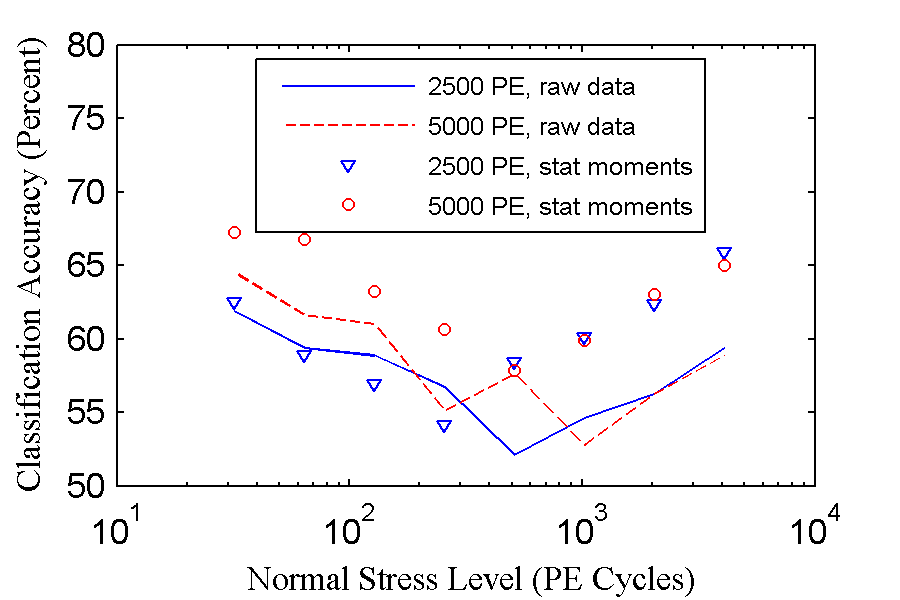
\includegraphics[width=\mywidth]{figs/svm_accuaracy.png} 
%\caption{Overall accuracy of trained SVMs vs. test data sets.}
%\label{fig:svm_acc} 
%\vspace{-0.1in}

%\end{center} 
%\end{figure}

\subsection{Retrieval without the Hiding Key}

\begin{figure} 
\begin{center} 
\includegraphics[width=\mywidth]{figs/group_accuaracy.png} 
\caption{BER as a function of the percentage of correct group members.}
\label{fig:group_ac} 
\vspace{-0.1in}

\end{center} 
\end{figure}

Without the hiding key, one can still attempt to extract the hidden
information. By estimating (through random guessing if necessary) which 
bits are grouped together,
an attempt at extraction could reveal data if enough of the estimate is
correct. Figure~\ref{fig:group_ac} shows the bit error rate versus the percentage
of correctly guessed group bits. 
%Bit error rate drops significantly as
%one approaches 60\% correct group member bits. 

With a large enough group and page size, it is difficult to %randomly
correctly guess enough of the group members. For our group size of 128, 
%the probability of correctly selecting even 10\% of a group out of 4,096 bits 
%is extremely low.
%Since the group number itself is important to the decoding
%process,it is not enough to get 10\% of any group in the randomly selected bits.
the probability that 
10\% (13) of the bits in a randomly selected group of 128 bits belong
to the desired group is approximately $\binom{128}{13} * (1/32)^{13}$; or 0.5\%.
As there are 32 groups of 128 bits in a 4,096 bit page, each bit has a 1/32 chance of
being in the desired group. Even at 10\%, the bit error rate is approximately
0.4. The chance of guessing 20\% of the bits in a randomly selected group drops
precipitously; it is 7.3e-11\%. In addition, an attacker would have to try
several group sizes.

Group size is a security parameter that one can adjust in order to provide
greater or lesser protection against brute force group selection.


\subsection{Erase Tolerance}

\begin{figure} 
\begin{center} 
\includegraphics[width=\mywidth]{figs/post_pe.png} 
\caption{Influence of post hiding PE cycles.}
\label{fig:postPE} 
\vspace{-0.2in}
\end{center} 
\end{figure} 

To test the erase tolerance of the scheme, we
deliberately stress the chip after hiding information on the chip. 
For this post-hiding stress, we program every bit of the page
to 0, in order to put the maximum stress on the bits.
The influence of post-hiding stress on the BER versus 
the number of PE cycles performed after hiding information
is shown in
Figure~\ref{fig:postPE}. From
the figure, we can see that the BER increases as the post PE
stress level increases. However, the BER of hidden information is quite
reasonable, even after hundreds of post PE cycles. For example, with 5,000 hiding PE
cycles, the BER is less than 10\% even after 500 post-hiding stress cycles.


\subsection{Different Flash Models}

To ensure that our scheme applies more generally, we tested
several different Flash memory models (shown in Table~\ref{tab:testedchips}).
On all of the chips, we were able to successfully hide and recover information.
We noticed that chips from the same manufacturer 
tend to perform similarly. For the Micron 2Gbit chips, 5
chips are tested using 10,000 hiding PE stress and 128-bit
groups. The mean BER for these five chips is 0.0030. The maximum
BER and minimum BER are 0.0041 and 0.0016, respectively. Chips
from different manufacturers perform differently. The tested Hynix
chip has a similar BER, 0.0021, as the Micron chips in the same
experiment. However, for the Hynix chips, page 0 is
different from other pages in a block and, in the decoding process, 
a different threshold $Th$ is needed 
to convert the average program time into 
the final binary bit for this page.
The tested Numonyx chip has a very large
gap for the group averages with the correct hiding key, making
its BER 0 in our experiment.

We also included a multi-level cell (MLC) chip in our testing, 
as these chips are commonly used. 
MLC chips map multiple bits to each memory cell. As a result, one needs to
know the mapping of bits to Flash cells to selectively stress certain cells.
%coding scheme for bits to
%achieve the highest stress difference
%between stressed groups and `unstressed' groups. 
For the Micron MLC chip we
tested, we only used the upper page in a pair of pages (as specified from the datasheet).
We programmed 0 to the bits which we want to stress and 1 to the rest of the bits.
Then, we programmed all of the bits to 1. Interestingly, we found that bits within 
a page split into a fast group and a slow group in this MLC chip, and only the faster programming
bits worked for information hiding. 
The MLC chip required significantly fewer PE cycles to achieve the same level of BER 
compared to the SLC chips. For example, we used 2,000 PE cycles for our experiments
and got a BER of zero -- there was a large gap between the more stressed and less stressed
groups. 
%An interesting observation is that when
%we characterized the program time using
%partial programming, the bits within a page splits into two groups depending on
%their partial program number and
%only the fast-programming group works for the hiding scheme. Nevertheless, we
%can use fewer PE cycles in MLC
%to achieve the same level of accuracy as in SLC, given other parameters are the
%same. We used 2,000 PE cycles for
%hiding in MLC. 
%The decoded bits have a large gap separation and the BER is zero
%in our limited testing. We believe
%it is caused by the larger programming stress difference between the highest
%threshold group and the lowest threshold
%group in MLC coding scheme. We also believe knowing more details than the
%datasheet about commercial MLC chips can help improve the scheme.



